%TODO
%update tables
%reread text


%\documentclass[10pt,iop]{emulateapj}
\documentclass[preprint]{aastex}
%\usepackage{rotating}
\usepackage{url}
\usepackage{multirow}
\usepackage{amsmath}
%\usepackage{graphicx}
%\usepackage[figuresright]{rotating}
%\usepackage{rotating}
%%\usepackage{natbib}

%\citestyle{aa}

%\bibliographystyle{apj_w_etal}

\newcommand{\etal}{{et al.\/}}
\newcommand{\Prob}{\mathtt{P}}
\newcommand{\logL}{\log\mathcal{L}}
\newcommand{\unit}[1]{\footnotesize #1}
\newcommand{\PAPER}{\mathrm{PAPER}}
\bibliographystyle{apj_w_etal}

	% End definitions

%\slugcomment{DRAFT: \today}

\shorttitle{Southern Hemisphere Flux Scale}
\shortauthors{Jacobs et al.}

\begin{document}

%\title{The Reionization flux scale in the Southern Sky}
\title{A Flux Scale for Southern Hemisphere 21cm EoR Experiments}
\author{
Daniel C. Jacobs\altaffilmark{1},
Aaron R. Parsons\altaffilmark{2},
James E. Aguirre\altaffilmark{3},
Zaki Ali\altaffilmark{2},
Richard F. Bradley\altaffilmark{4,5,6},
Chris L.  Carilli\altaffilmark{7},
David R. DeBoer\altaffilmark{8},
Matthew R. Dexter\altaffilmark{8},
Nicole E. Gugliucci\altaffilmark{5},
Pat Klima\altaffilmark{5},
Dave H. E. MacMahon\altaffilmark{8},
Jason R. Manley\altaffilmark{9},
David F. Moore\altaffilmark{3},
Jonathan C. Pober\altaffilmark{2},
Irina I. Stefan\altaffilmark{10},
William P. Walbrugh\altaffilmark{9}}

\altaffiltext{1}{School of Earth and Space Exploration, Arizona State U., Tempe, AZ}
\altaffiltext{2}{Astronomy Dept., U. California, Berkeley, CA}
\altaffiltext{3}{Dept. of Physics and Astronomy, U. Pennsylvania, Philadelphia, PA}
\altaffiltext{4}{Dept. of Electrical and Computer Engineering, U. Virginia, Charlottesville, VA}
\altaffiltext{5}{National Radio Astronomy Obs., Charlottesville, VA}
\altaffiltext{6}{Dept. of Astronomy, U. Virginia, Charlottesville, VA}
\altaffiltext{7}{National Radio Astronomy Obs., Socorro, NM}
\altaffiltext{8}{Radio Astronomy Lab., U. California, Berkeley, CA}
\altaffiltext{9}{Square Kilometer Array, South Africa Project, Cape Town, South Africa}
\altaffiltext{10}{Cavendish Lab., Cambridge, UK}

\begin{abstract}
We present a first catalog of broad-band spectral measurements from the 
Donald C. Backer Precision Array for Probing
% XXX ARP: was irina "first"?  and maybe "catalog"
the Epoch of Reionization (PAPER) in South Africa observed in July and
September of 2011.  In order to reduce the impact of beam calibration, which proves to
be a difficult endeavor for transit telescopes such as PAPER, on the determination
of source spectra, we have focused on calibrating sources in a narrow declination range.
Since each source follows a nearly identical path through the primary beam, this
restriction allows beam calibration to be nearly eliminated as a source of error,
yielding a dramatic improvement in the accuracy of source spectra measured in the 
100--200-MHz band that is receiving renewed attention by experiments seeking to
measure 21cm emission from the Epoch of Reionization (EoR).
Based on the variation in our data and the estimated error in the absolute
flux scale we bootstrap from multiple bright sources, we estimate PAPER measurements
of sources above XXX Jy to be accurate to 3.2\%.
When combined with catalog data at other frequencies, these data constrain parameters of
a power-law model for flux density with an uncertainty of 2.4\%.
% XXX ARP: this must again be dependent on source strength and location.
This accuracy is limited by the uncertainty in the catalog measurements we use
to estimate an absolute flux scale, and represents 
an order of magnitude improvement over previous measurements in this band.  
Comparing with prior measurements, 45 out
of 58 sources observed are found to confirm and refine a power-law model for flux density.
This includes Pictor A, which provides a key flux reference for PAPER's EoR
power spectrum analysis.
\end{abstract}

\keywords{dark ages, reionization, first stars --- catalogs --- instrumentation: interferometers}

Numerous radio telescopes are now exploring the prospects for using
measurements of highly redshifted 21cm emission to inform our understanding of
cosmic reionization in the redshift range $6< z<12$, corresponding to radio
frequencies below 200 MHz (see reviews in
\citealt{Furlanetto:2006p2267,Morales:2010p8093,Pritchard:2012p9555}) .  These
include telescopes aiming to measure the global temperature change of 21cm
emission during the Epoch of Reionization (EoR), such as the Compact
Reionization Experiment (CoRE) and the Experiment to Detect the Global EoR
Signature (EDGES; \citealt{Bowman:2010p8546}), and interferometers aiming to
measure the power spectrum of 21-cm EoR emission, such as the Giant Metre-wave
Radio Telescope (GMRT;
\citealt{Paciga:2011p9470,Paciga:2013p9627})\footnote{\url{http://gmrt.ncra.tifr.res.in/}},
the LOw Frequency ARray (LOFAR;
\citealt{Yatawatta:2013p9699})\footnote{\url{http://www.lofar.org/}}, the
Murchison Widefield Array (MWA;  \citealt{Bowman:2012p9138};
\citealt{Tingay:2013p9022}))\footnote{\url{http://www.mwatelescope.org/}}, and
the Donald C. Backer Precision Array for Probing the Epoch of Reionization
(PAPER; \citealt{Parsons:2010p6757,Parsons2013b})\footnote{\url{http://eor.berkeley.edu/}}.

As such, there has been a renewed interest in the spectral and spatial variation of
foreground emission in the 100--200 MHz frequency band that covers
the $z=6$--13 redshift range expected to encompass reionization
\citep{furlanetto_et_al2006}.
In particular, the spectral properties of extra-galactic point-sources are important
both because they are valuable calibration references
and because they are strong foreground emitters that must be removed from 21-cm EoR measurements.
With the sparse availability of measured foreground properties in the
100--200-MHz frequency band over large areas of the sky \citep{deolivieracosta_et_al2008}, continued
foreground characterization is a
vital step en route to any 21-cm EoR detection.
Both PAPER and the MWA are located in the southern hemisphere at radio quiet
reserves being prepared for the upcoming Square Kilometer Array.  At these low
frequencies the Southern sky is much less well known than the North, with the
most extensive surveying work being conducted  by the EoR experiments
themselves \citep{Jacobs:2011p8438,Williams:2012p8768}.
  
% XXX is the "eor science" part necessary?  this isn't a paper on eor
Neutral hydrogen is visible during reionization as $\sim$30mK excess surface
brightness over the CMB punctuated both spectrally and spatially by regions of
zero emission.  This patchy signal is predicted to be visible everywhere on the
% XXX ARP: don't like description of EoR signal as "surface brightness"
sky at size scales up to degrees, or about $0.1$cMpc$^{-1}$.   To increase the
surface brightness sensitivity without building costly dishes, MWA, PAPER and
LOFAR have chosen to use combinations of phased and/or correlated dipoles. By
design also cover much wider fields of view ($>10$\arcdeg) and bandwidths
($\sim 100$\% fractional) than traditional dish telescopes.   As the elements
% XXX what about GMRT?
can not be physically pointed, the apparent flux scale varies across the sky.
This direction dependent gain is currently uncertain to 20\% or higher
\citep{Jacobs:2013p9713}.  The ideal solution is to use a wide-grid of
well-known calibrators to map the primary beam and set the flux scale.  
% XXX don't go to "ideal solution" just yet
% XXX ARP: add importance of accurate flux vs. frequency (Parsons et al. 2012, etc.)

%The position dependent gain varies for each instrument.   LOFAR and MWA have a range of electrically steerable beams each with a different shape. For MWA and LOFAR, the number of high quality calibration sources is more important.  PAPER has a single broad, 45\arcdeg wide, primary beam; sources at nearby declinations sample the same primary beam many times.
% This will in turn provide a wide base to assess the accuracy of the primary calibrator which sets the overall amplitude of the EoR power spectrum.  




However, catalog source fluxes at 150MHz are also inaccurate to the 20\% level,
particularly at southern declinations ($\delta<-20$\arcdeg) . Historically, the best
EoR band data were by \citet{Slee:1995p7541} with Culgoora Circular
Array\footnote{Known during daylight hours as Culgoora Radio Heliograph} and
various higher frequency measurements with Parkes.  These data are typically
uncertain to 10\% or higher and provide little coverage of the EoR band beyond
a single narrow-band data point. 

PAPER, in its maximum redundancy configuration, has a very broad beam with
% XXX need background on minimum/maximum array configurations
large regular grating side-lobes and is therefore limited to using the few
sources above $\sim$50 Jy for flux calibration. The best calibrator for most
% XXX qualify "best"
observations is Pictor A. For this source the current best EoR band measurement
is uncertain to 12\% and appears to imply spectral flattening in the EoR band
\citep{Perley:1997p9312}.

More recent surveys include narrow-band surveys by the GMRT and Mauritius, a
deep survey of the region near Hydra A by the 32 antenna MWA prototype
\cite{Williams:2012p8768} and a wide field survey by PAPER, also with 32
elements \cite{Jacobs:2011p8438}. Several sub-channels were provided in the
Williams catalog, though with 60-80\% error bars ---large compared to the 30\%
uncertainty on their wide band measurements.  The latter cover the band and
spatial scales relevant to EoR measurements but are limited by the accuracy of
the primary beam \citep{Jacobs:2013p9713}.

A method for decoupling uncertain fluxes from the uncertain beam has been
described by \citet{Pober:2012p8800}. In simulation the method was able to
achieve 3 to 10\% accuracy in measuring the primary beam, depending on the
number of antennae and other variables. The Pober method emphasized the need
for many repeated measurements of each alt-az pointing. Further investigation
is under way to improve and implement this method and would be greatly aided by
the availability of precise flux measurements unaffected by primary beam
uncertainty. This paper reports a set of flux measurements where a primary beam
model has not been used to estimate the flux, but instead are directly
calibrated to a single calibrator making the track through the beam.



The spectra were measured by PAPER, a dedicated EoR experiment 
that employs drift-scanning, dual-polarization dipole antennas 
tuned for efficient operation over a 120--170-MHz band located in the South African Karoo desert
on the Square Kilometer Array
South Africa (SKA-SA) reserve, 100km north of the small town of Carnarvon.
The PAPER array has grown from 16 elements deployed in early 2009 to a
64-element imaging array in 2011 (see Figure \ref{fig:antpos}). Since November 2011 it has been arranged in a maximally redundant grid configuration to make deep power spectral integrations \citep{Parsons:2012a}.
\begin{figure*}\centering
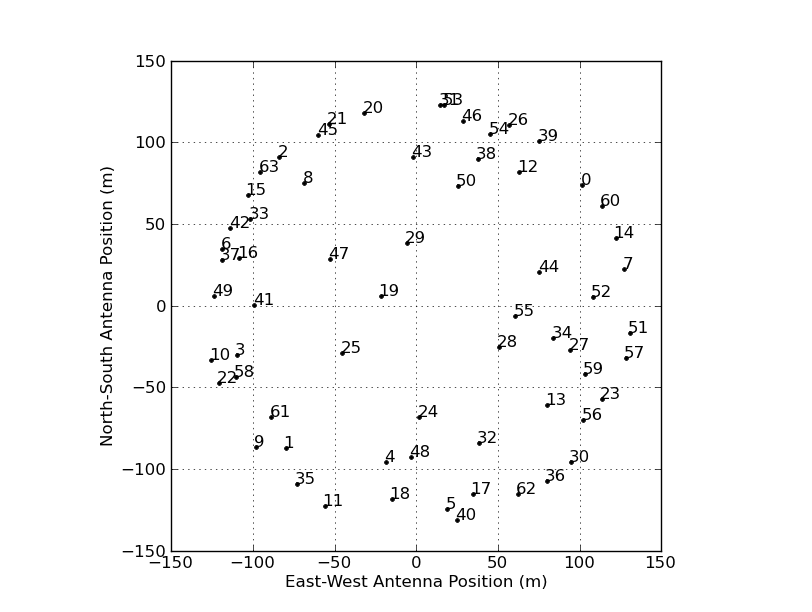
\includegraphics[width=0.85\columnwidth]{plots/antpos.png}
\caption{Antenna position in the 64-antenna, minimum-redundancy PAPER array configuration at the Karoo Radio Observatory site in South Africa used for these observations.
% XXX add brief summary of observations.
}\label{fig:antpos}
\end{figure*}

In this paper our primary goal is to provide a subset of accurate fluxes
suitable for EoR power spectrum and catalog calibration.  After recording the
data used in this paper, PAPER was reconfigured into a redundant layout
optimized to detect a small number of power spectrum bins at high precision, an
arrangement which trades imaging dynamic range for power spectrum sensitivity.
As such it is only able to easily distinguish the very brightest sources on the
sky a step necessary for setting the overall flux scale \citep{Parsons2013b}. Of these, Pictor A is
one of the most useful, being bright, minimally resolved and far from from
confusing structure. 

The data  include new measurements of Pictor A that are uncertain to 3.5\%,
close to the level of the most precise higher frequency measurements by
\citet{Wills:1975p9314}. Using these new measurements we update the spectral
calibration model to an accuracy of 2.5\%. As validation of this method, we
also measure a selection of 58 additional sources at the same Declination.  The
primary beam is calibrated using a single common source (J2331-416), thus
limiting the declination probed to $-45 \pm 5$\arcdeg.  The flux scale is set
by Monte Carlo fitting to a subset of sources, all of which are calibrated to
the Baars et al scale. In \S\ref{sec:Observations} we describe the instrumental
setup, observations and analysis method followed. In \S\ref{sec:fits} we
compare the spectra with available data followed by conclusions in
\S\ref{sec:Conclusion}.

%This declination limit removes the necessity of correcting for a primary beam model and allows us to calculate more precise fluxes that provide a reference standard for future work.

\section{Approach}

% XXX write this section

% XXX incorporate
%Given these shortcomings in the literature, we felt it prudent to examine-Pictor A directly.  We use data observed on JD2455747 
%from a 64-antenna single-polarization deployment of the 
%PAPER array in a minimum redundancy configuration that is more suited for imaging.  The details
%of these observations and their calibration are given in \citet{pober_et_al2013}.  In order to ensure that 
%errors in
%the beam model did not skew our result, we chose a set of calibrator sources near in declination
%to Pictor A that would follow nearly identical tracks through the primary beam.

% XXX incorporate
%To measure the spectrum of each source, we apply per-antenna phase and gain cal
%brations established-via self-calibration and remove
%the known dependence of amplifier gain and cable attenuation on ambient temperature was corrected
%using measured temperature data and temperature coefficients that were characterized in
%laboratory measurements \citep{parashare_bradley2009} and confirmed in field-measurements \citep{pober_et_al2012}.  For each source, we phase to the source 
%osition
%and sum over 
%all baselines greater than 20 wavelengths in length.
%A fringe-rate filter is applied to the resulting
%beam to suppress beam sidelobes where sources introduce variations that deviate more than 
%$\pm$0.1 mHz from the fringe rate of the source in question.

% XXX incorporate
%To derive a source spectrum from each drift-scan source profile, we compute a weighted average using
%weights derived from a model of
%PAPER's primary beam response as an effective approximation of inverse-variance weighting
%\citep{pober_et_al2012}, and averaging over the time series for each source.  Each output source spectrum
%represents a best estimate given the limitations of the beam model and flux calibration that were established
%up to this point.  To further improve these estimates, we derive an additional frequency-dependent gain parameter,
%smoothed on 10-MHz scales,
%that brings the spectrum of J2331-416 into closest agreement with a power-law spectrum of
%$S_{150}=31.9\ {\rm Jy}$, $\alpha=-0.69$ that represents the best fit to measurements below 1 GHz.
%This additional gain factor was applied to all measured spectra, including that
%of Pictor A.  The expectation is that, since all sources at similar declinations follow similar tracks 
%through the PAPER beam, any errors present in the original measured spectra as a result of differences between
%the simulated and actual beam response should be absent in the ratio between source spectra, and therefore
%should be corrected by the applied gain factor.

% XXX incorporate
%Finally, because Pictor A is resolved at the 20\% level on the longest (300m) East-West PAPER baselines, we 
%use per-baseline estimates of resolution weights to down-weight and correct for resolution effects.  To estimate
%resolution weights, we use the 90cm map of Pictor A presented in \citet{perley_et_al1997}.  Averaged over all
%the baselines in the array, the inclusion of resolution effects changed the measured flux by less than 5\%.

 
 \section{Observations and Data Reduction}
 \label{sec:Observations}

 Measurements are derived from observations using  the east-west dipole arms of
64 PAPER antennas deployed in the Karoo Radio Observatory site in South Africa
(see Figure \ref{fig:antpos}).  A 100-MHz band from 100-200MHz was correlated
with 2048 frequency channels and integrated for 10.7 seconds before
visibilities were stored.  Observations included here on  July 4, 2011, running
from JD2455748.17 to JD2455748.72. and October 17, 2011 running from
JD2455852.2 to JD2455852.6.  In both seasons two antennas were omitted owing to
malfunctioning signal path. This 20 hour long combined dataset provides
observations provides complete hour angle coverage for the entire 24 hours of
Right Ascension. The July portion of the dataset comes from the same observing
campaign described by \cite{Pober:2013p9567} and \cite{Stefan:2012p9707}. 
%July (\#40,\#55), September (\#7,\#28) 

%COMPRESSION
\textbf{Compression}\\

In pre-processing, we use delay/delay-rate (DDR) filters
\citep{Parsons:2009p7859} to identify radio-frequency interference (RFI)
events, and as part of a data compression technique that reduces data volume by
over a factor of 40.  A more detailed description may be found in Appendix A of
\cite{Parsons2013b}, which uses the same compression method on PAPER power
spectrum observations. Here we summarize the process.

First, we remove known RFI transmission bands and analog filter edges, and then
flag outliers at 6$\sigma$ to remove RFI events.  Next, we suppress foreground
emission by applying a DDR filter to remove delays and delay-rates within the
horizon limit of a 300-m baseline (the maximum length of any PAPER baseline).
We derive a second set of RFI flags by masking 4$\sigma$ outliers in these
residuals and apply these flags back to the unfiltered data.  Finally, we
compress the data by applying a DDR filter preserving emission within the
horizon limit of a 300-m baseline, deconvolving to suppress flagging artifacts,
and down-sampling the result in time/frequency domain to the critical Nyquist
rate of the DDR filter.  The result is that the 2048 original frequency
channels become 203, and the 60 original time samples per 10-minute file become
14. 

% XXX merge with below
%Removed RFI by flagging samples in each frequency channel versus time that exceed the mean amplitude by 4-sigma
%after performing a time derivative.  Also flagged samples in each integrated spectrum that exceeded the
%mean amplitude across the spectrum by 6-sigma after performing a frequency derivative.  For efficiency, flagging
%was derived using only the subset of baselines involving a fiducial antenna.
%Frequencies below 120 MHz and above 180 MHz were also flagged, owing to roll-off of analog response.
%After RFI flagging, frequency channel resolution was decreased by a factor of four by summing channels.


%CALIBRATION
\textbf{Antenna calibration}\\

% XXX time-dependent calibration is critical.  modify paragraph below
Quantization gain through the correlator was linearized \citep{parsons_et_al2008}.
Finally, measurements of ambient temperature versus time near the balun amplifier of a fiducial antenna and near
receiver amplifiers were used to divide out the predicted gain variation versus temperature that these amplifiers
are known to exhibit.  A predicted gain profile was drived using coefficients characterized in
laboratory measurements \citep{parashare_bradley2009} and
confirmed in field measurements \citep{pober_et_al2011} of $H_{\rm balun}=-0.024$ dB/K, $H_{\rm recvr}=-0.045$
dB/K, and $H_{\rm cable}=-0.018$ dB/K for 150m-long cables.  Because cable temperatures were not measured
during these observations, the cable temperature was assumed to be the same as the measured balun temperature.


Antennae delays and amplitudes were found by fitting a point source visibility
model to Centaurus A, Pictor A, and Fornax A.  Each source is imperfectly
modeled by a single point-source, but the solution differences are minimized by
averaging over the three independent solutions. These same calibration
solutions have been successfully applied in \citet{Pober:2013XXX} and \citet{Stefan:2013:XXX}.
for power-spectrum analysis of foregrounds and imaging of Centaurus A, respectively.

% XXX differentiate amp cal here from spectral cal that comes later.

%BEAMFORMING,FILTERING, AVERAGING
\textbf{Source Selection}\\

In order to ensure that errors in
the beam model did not skew our result, we chose a set of sources near in declination
to Pictor A that would follow nearly identical tracks through the primary beam.
A list of these 
sources is given in Table \ref{tab:src_spec}, with the spectra measure by PAPER
illustrated in Figure \ref{fig:src_spec}.  These sources were chosen on the basis of brightness and
proximity in declination to Pictor A.
% XXX merge this with paragraph below

To provide a basis for establishing the accuracy of the Pictor measurement we
measured more sources.  Specifically, we choose sources from the Molonglo
Reference Catalog \cite[MRC]{Large:1981p7798} that are within 5\arcdeg in
declination of a common calibrator (J2331-416) and have a flux extrapolated
from 408MHz greater than 10Jy assuming a power law spectral index of
-1.\footnote{Most radio sources in this band have power law spectra $S(\nu) =
\left(\frac{\nu}{\nu_0}\right)^\alpha$.  The 5\arcdeg distance between source
and calibrator was chosen as a balance between number of sources included and
the known smoothness of the beam.   The average spectral index for radio
sources in this band is $-0.8$.} This selection contains 62 sources in a narrow
stripe that passes through the majority of the southern EoR fields, much of the
galaxy and Centaurus A.



\textbf{Beamforming}\\

Spectral time-series are computed by beam-forming to the selected sky
locations. A beam is formed by phasing baselines to the desired location and
summing over baselines.  
%Samples were only included if there was a calibrator sample within 5\arcdeg in altitude/azimuth.   By using both seasons of data we were able to match all measurements with calibrator measurements, making this cut moot. 

% XXX incorporate paragraph below
%As the sky drifts through the primary beam of PAPER antennas, widely
%separated points will be observed with substantially different gains and
%so will require different data weightings to optimize SNR.
%Drift-scan observations of sources were divided by the calibrated beam response in the
%direction of the source as a function of time.  Spectra were calculated by averaging over
%time, weighting data at each time step by the square of the 150-MHz beam response in the source direction.
%Since noise and systematics relating to source observations are expected to be approximately constant
%versus time, while source amplitude is proportional to beam response, this weighting
%is an effective approximation of inverse-variance weighting \citep{pober_et_al2011}.

% XXX exclusion of minimum uv spacing?


 These complex spectra are then delay-delay rate filtered to remove spectrally
smooth sources far from phase center \citep{Parsons:2009p7859} (cf the LOFAR
de-mixing approach \cite{Offringa:2012p9691})  producing a time dependent
spectrum. This is then averaged in time,  weighting by a model of the primary
beam. This down-weighting, or multiplying by the primary beam, should be
clearly distinguished from up-weighting, which we are at pains to avoid.
Weighting by another factor of the primary beam is an effective approximation
of inverse-variance weighting \citep{Pober:2012p8800} and reduces the
contribution of noisy low elevation measurements.  The result is equivalent to
a very long earth rotation synthesis image with a single image pixel. When
combined with the filtering it is a robust and simple method for measuring
spectra of unresolved sources. 

% XXX incorporate paragraph below
%To measure the spectrum of each source, we apply per-antenna phase and gain cal
%via self-calibration and remove
%the known dependence of amplifier gain and cable attenuation on ambient tempera
%using measured temperature data and temperature coefficients that were characte
%laboratory measurements \citep{parashare_bradley2009} and confirmed in field
%measurements \citep{pober_et_al2012}.  For each source, we phase to the source 
%and sum over 
%all baselines greater than 20 wavelengths in length.
%A fringe-rate filter is applied to the resulting
%beam to suppress beam sidelobes where sources introduce variations that deviate
%$\pm$0.1 mHz from the fringe rate of the source in question.




\begin{figure}
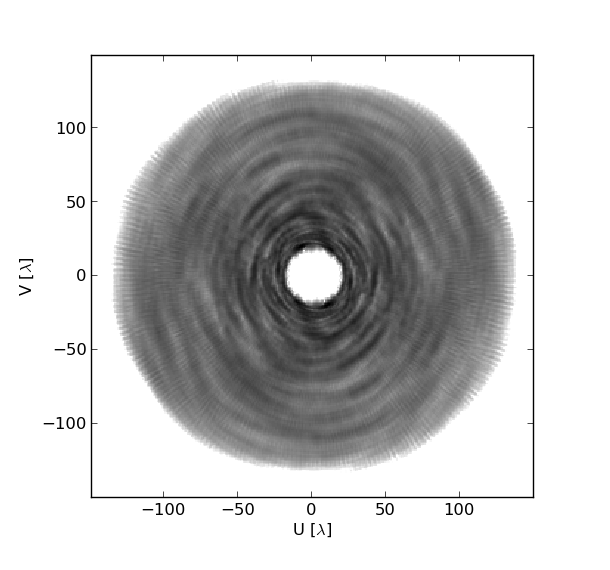
\includegraphics[width=0.9\textwidth]{plots/PicA_Oct2011_uv_coverage.png}
\caption{The effective uv coverage, showing the relative contributions of each baseline when beam-forming on Pictor over a 9.6 hour synthesis in the October observing session. \label{fig:uv_coverage}}
% XXX unclear whether amplitudes include our model of Pic A, or are even actual data vs. weights
\end{figure}

The beam-forming method assumes the target is a point source. Our primary
target, Pictor A, is slightly resolved by PAPER, and merits closer attention.
Pictor A is a double-lobed radio galaxy with a main lobe separation of
7\arcmin. As we see in Figure \ref{fig:pic_perley}, it is nearly unresolved by
PAPER's 15\arcmin synthesized beam. However, given the high SNR of the
observations, resolution effects are observers, in a slight decrease in flux on
the longest ($\sim$300m) baselines. We account for this by weighting baselines
in the beam form step according to a model of structure observed by
\citet{Perley:1997p9312} at 330MHz, which they found to be consistent with
their more limited 74MHz images as well as the detailed high frequency maps.
The normalized image is Fourier transformed and sampled at the desired uv
spacing by spline interpolation. These samples are used to weight each baseline
contribution in the baseline sum. The result is an estimate of the total
integrated flux for Pictor A. Where the resolution is highest, at the top of
the band, the correction is 3\%. At the bottom of the band, where the
resolution size has grown to 19\arcmin, the correction is only 0.6\%. The
resulting spectrum is shown in Figure \ref{fig:pic_spectrum}a.

\begin{figure}
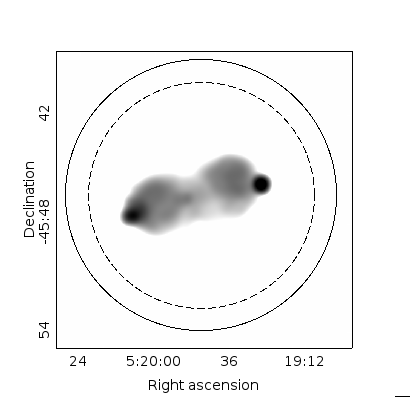
\includegraphics[width=0.96\textwidth]{plots/picA_Perley.png}
\caption{
Pictor A imaged at 330MHz by the VLA \citep{Perley:1997p9312}. Black circle
indicates PAPER resolution at the 150MHz, dashed, the resolution at 185MHz.  To
correct for the small residual structure in the PAPER measurements we
interpolated the PAPER baselines in the uv plane. At the highest frequency this
% XXX "interpolated" needs to be clarified
led to a 3\% correction, at the lowest frequency, 0.6\%.
\label{fig:pic_perley}}
\end{figure}

%BANDPASS CALIBRATION
\textbf{Spectral calibration}\\
\label{sec:Calibration}

% XXX selection of calibrator sources

The gain of each channel is the product of an overall instrumental passband and
the spectral dependence of the primary beam in the direction of the source.
Sources sharing the same track through the primary beam will have the same
average spectral gain function resulting from frequency dependent primary beam
attenuation.   We matched each measured source spectrum time sample to the
nearest sample (in altitude/azimuth) of a calibrator source
(J2331-416)\footnote{This source was chosen for the amount of data found in the
literature and the apparent smoothness of the spectrum.}.  We then, average the
% XXX clarify why one source used here, and more sources later 
two matched data streams in time.  Since both tracks make the same slice
through the primary beam, they will have the same average effective gain.
Assuming a power law model for J2331-416 (33Jy $\alpha=-0.76$), we compute a
bandpass gain.  After calibrating the raw 203 channel spectra with this
bandpass, we average into 10MHz sub-bands between 120 and 180 MHz, computing
the standard deviation as an estimate of the error. 

% XXX merge this with above
%To further improve these estimates, we derive an additional frequency-dependent gain parameter,
%smoothed on 10-MHz scales,
%that brings the spectrum of J2331-416 into closest agreement with a power-law spectrum of
%$S_{150}=31.9\ {\rm Jy}$, $\alpha=-0.69$ that represents the best fit to measurements below 1 GHz
%\citep{slee1995,kuhr_et_al1981,large_et_al1981,burgess_hunstead2006}.
%This additional gain factor was applied to all measured spectra, including that
%of Pictor A.  The expectation is that, since all sources at similar declinations follow similar tracks 
%through the PAPER beam, any errors present in the original measured spectra as a result of differences between
%the simulated and actual beam response should be absent in the ratio between source spectra, and therefore
%should be corrected by the applied gain factor

\textbf{Catalogs}\\

Data for prior comparison was pulled from two major sources. Catalog values for
Pictor A, and the flux calibration sources were pulled directly from the
NASA/IPAC Extragalactic Database (NED)
\footnote{\url{http://ned.ipac.caltech.edu/}}. Cross-matching radio sources
between bands is made difficult by changes in resolution, spectral curvature,
and resolved multi-scale structure.  For a small number of sources these
problems can be ameliorated by inspection of the spectra, source names,
coordinates,  and originating publications. However for a large sample of
sources this becomes unwieldily and prone to error. Thus for the larger number
of samples we make use of the Vollmer et al meta-catalog which takes pains to
match multi-wavelength observations \citep{Vollmer:2010p6422}.
% given the known source dimensions and spectral properties as well as telescope bandwidth and spatial resolutions. 


\textbf{Flux Scale}\\
\label{sec:flux_scale}

At this stage each source flux is tied to a model fit on the catalog values of
J2331-416. The accuracy of this fit and the implied uncertainty in the flux
scale limits the accuracy of the PAPER measurements..  To refine the flux
scale, we bootstrap a single global flux scale correction factor using 5
sources selected for their brightness, spectral linearity and data
availability\footnote{Calibration sources:
2250-412,2331-416,2140-434,0007-446,0704-427}. To build a more complete
spectral model we go beyond the data found in SPECFIND, using all spectral
measurements below 2GHz found in the NED database.  These catalog measurements
are primarily by Parkes, and Molonglo with the best precision coming from the
Wills fluxes at 538 and 634 MHz (when available). Where error bars are not
given, we assume uncertainty of 25\%. 

As described in the Appendix, we fit spectral index models for all sources
(using catalog data) simultaneously with a global PAPER flux scale factor
(using the PAPER data). We fit the model using a Markov Chain Monte Carlo
sampler to sample the posterior probability of PAPER data ($SPAPER_{\nu}$) and
catalog values ($Scat_{\nu}$) given a spectral index model for each source and
a global flux scale factor ($g$) ($S_\PAPER^\textrm{calibrated} = g S_\PAPER$).
The resulting flux scale distribution function is shown in Figure
\ref{fig:gain}. The 76\% confidence limit on this flux scale, relative to the
J2331-413 calibration, is  $-0.01 ^{+0.11}_{-0.17}$ dB, or a 3.24\%
multiplicative error on every calibrated PAPER measurement.  


The calibrated spectra are plotted in Figures \ref{fig:srcs1},\ref{fig:srcs2},
\& \ref{fig:srcs3} and the data are listed in Table \ref{tab:data}.  See the
Appendix for details on this fitting procedure and definition of terms.  The
resulting Pictor A spectrum ranges in precision from 6.5\% at 125MHz to 4.7\%
at 185MHz. At least half of this error is due to uncertainty in the flux scale.  
%\footnote{Of the 315 data points in this catalog, 7 fluxes points are negative. All three occur quite close to Centaurus A, which has large structure on degree scales in this region and is the brightest sources in the sky. These sources have been flagged and removed from further analysis.}

%The Pictor track is calibrated to 2331-416 ($S_{150}=33.8$Jy,$\alpha=-0.76$) and the Hydra A track to 0231-126 ($S_{150}=21$Jy,$\alpha=-0.7$).  
%    cal['0213-132'] = 21 * (fq/.150)**-0.7  
%    cal['1932-464'] = 93.7 * (fq/.150)**-0.82 
%    #cal['2331-416'] = 31.9 * (fq/.150)**-0.69
%    cal['2331-416'] = 33.9 * (fq/.150)**-0.76
%COMPARISON WITH DATA

 \section{Spectral Results}
 \label{sec:fits}

The primary purpose of this observation is to produce a high quality Pictor A
% XXX need to coordinate "primary purpose" here with abstract and intro motivation
spectrum. As a verification measure we have observed many other sources at the
same declination for comparison against previous observations.  Our comparison
metric will be the degree to which the PAPER data are consistent with previous
observations,given a model and, if consistent, they improve on the precision of
our spectral model parameters.

To compare with observations at other frequencies we must assume a spectral
model. The prevailing spectral model for low frequency radio sources is a
single power law due to synchrotron emission, though curvature or other
deviation from a power-law is not-uncommon.   To establish a baseline model, we
fit a spectral model to prior catalog data from the spectrally and spatially
cross-matched meta-catalog by \citet{Vollmer:2010p6422} using the MCMC method
described in \S \ref{sec:flux_scale} and the Appendix. Confidence contours for
these fits are shown in grey in Figs. \ref{fig:SI_contour_1} -
\ref{fig:SI_contour_4}.  In general these are lower limits on the possible
precision, as the Vollmer catalog emphasizes minimization of cross-match error
but at the cost of excluding data points.  The fit is then performed again with
both PAPER and catalog data, shown in black on the same Figures. The values are
given in Table \ref{tab:fits}. 

%0008-421#
%1243-412#
%1247-401#
%1315-460
%TODO round up the source counts

In the 59 sources measured, four demonstrated poor convergence fitting a single
spectral index to both the PAPER data and prior catalog data. In three
cases\footnote{1243-412,1247-401,1315-460} %TODO update these sources are in
the Centaurus A/galactic plane region. Though the beam forming method provides
relatively high dynamic range of $\sim$100:1 it is unable to distinguish
between these sources and the bright diffuse Centaurus and galactic structure.
The last source, 0008-421, was not detected by previous PAPER observations and
exhibits flattening at higher frequencies, most likely due to synchrotron
self-absorption \citep{Jacobs:2011p8438} .  The remaining 94\% MCMC chains
arrived at a stable posterior distribution. The spectral index parameters for
these chains are given in table \ref{tab:fits}.

Inspecting the confidence contours we find that, for the vast majority ($\sim
75$\%), the PAPER measurements confirm the power law extrapolation from higher
frequencies. The remaining 25\% either A) have large PAPER error bars and
therefore provide no new information or B) do not agree with the spectral index
model.  To understand where most measurements fall on this spectrum we
numerically quantify the overall model improvement derived from the addition of
the PAPER data as 
\begin{align}
\textrm{Improvement} &= \left(\textrm{Precision increase}\right) \left(\textrm{Catalog agreement}\right)\\
&= \left(\frac{1}{Area(\textrm{PAPER})} - \frac{1}{Area(\textrm{Cat})}\right) \left( Area(\PAPER \cap \textrm{Cat}) \right)
\end{align}
% XXX This equation is yucky

We quantify the fit {\em precision increase} as the change in the contour
figure of merit, defined as the inverse area of the confidence contour.
Meanwhile, {\em catalog agreement} is the fraction of the PAPER confidence
interval that overlaps the catalog confidence interval.  Thus, for example, in
a PAPER fit that overlaps the catalog confidence contour by 41\% but increases
in precision (confidence area shrinks) by a factor of 3, the resulting {\em
improvement} will be 0.123.  

In these sources, the improvement index ranges from a max of 6.9 to -0.022.
10\% of sources showed negative improvement, suggesting that PAPER data have
added to uncertainty (see Figure \ref{fig:SI_contour_bad}). 12\% of sources
have exactly zero improvement, which indicates that the PAPER data have pulled
the fit far from the model preferred by the catalog data (see Fig.
\ref{fig:SI_contour_new}).  The spectral models of these sources have not been
included in Table \ref{tab:fits}.  The remainder of the spectral fits are
included for completeness, but given the range of quality found, particularly
near the Galactic plane and Centaurus A, should be used with utmost caution.

However, the majority of source 78\% have positive improvement index,
indicating strong confirmation of the extrapolated spectrum (see Figures
\ref{fig:SI_contour_1} - \ref{fig:SI_contour_4}).  Pictor A is in the middle of
this group  with an improvement of 0.39 ---only 14 sources show stronger
confirmation.  The flux model is $S150=$388 $\pm$ 9.4Jy, $\alpha=-0.77\pm0.02$.
% XXX need more detail here.  This is the crux of what is done.
The combination of several independent PAPER data points near 150MHz with
previous catalog measurements results in this estimated uncertainty of 2.4\%.
This uncertainty is dominated by agreement between the 2 Wills measurements
near 600MHz which are accurate to 2\% and the five PAPER measurements, which
are accurate to ~5\%.


 \section{Discussion and Conclusions}
 \label{sec:Conclusion}
 
Direct measurements of the Pictor A spectrum are key to correctly setting the
flux scale of PAPER and other EoR experiments. Existing EoR band measurements
are accurate to 20\% implying a 40\% uncertainty in the absolute power spectrum
level.  Here we have provided new measurements of Pictor A that are accurate to
2.4\%;  388 $\pm$ 9.4Jy on the \citet{Baars:1977p9678} scale. The PAPER
measurement has a precision of $<$1\%; the majority of the uncertainty comes in
setting the absolute flux scale from prior data.  

We also take advantage of multiple PAPER observations to measure the next  61
brightest, previously cataloged, sources. These sources are distributed over
the full 24 hours of Right Ascension coverage but are within 5 degrees
declination of Pictor A.  Using a Bayesian analysis we conclude that most of
these are consistent with previous measurements and provide useful new
constraints. However, in the remainder, the simple spectral model fails to
adequately describe the data. In most cases the proximity to bright or extended
structures implies side lobe contamination.  Therefore, though we include the
model parameters, they are not meant to be definitive, but provide confidence
that the reported PAPER flux values are on the correct global scale.

% XXX need more discussion


\begin{figure*}
\centering
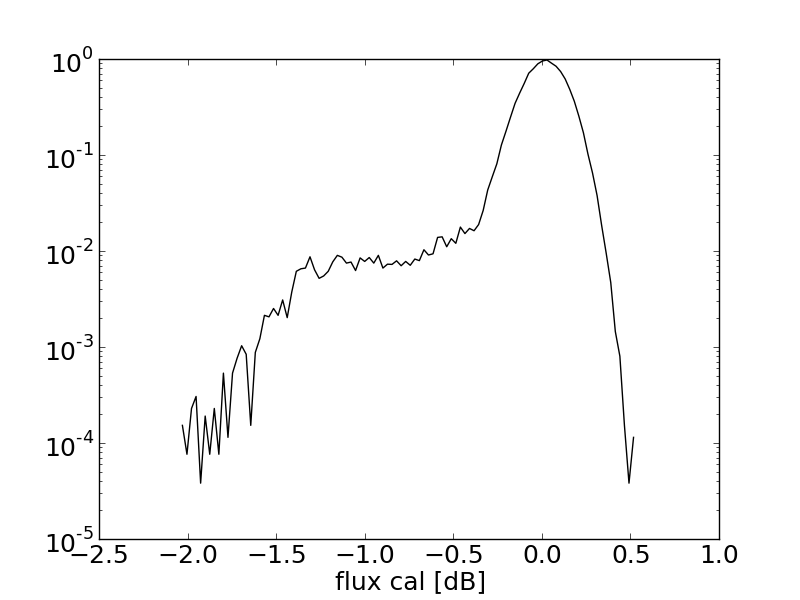
\includegraphics[width=0.9\textwidth]{plots/2250-412_2331-416_2140-434_0007-446_0704-427_gain_mcmc_chain_gain_conf.png}
\caption{
The marginalized PAPER flux scale factor posterior probability distribution
function bootstrapped from the NED database listings for
2250-412,2331-416,2140-434,0007-446 and 0704-427 below 2GHz.
\label{fig:gain}}
\end{figure*}

\begin{figure*}[htbp]
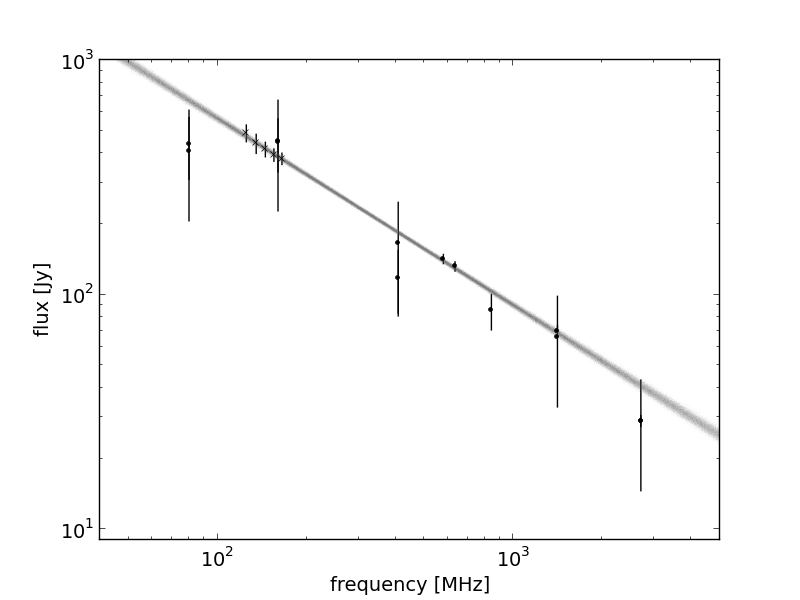
\includegraphics[width=0.49\textwidth]{plots/pictor_spectrum.png}
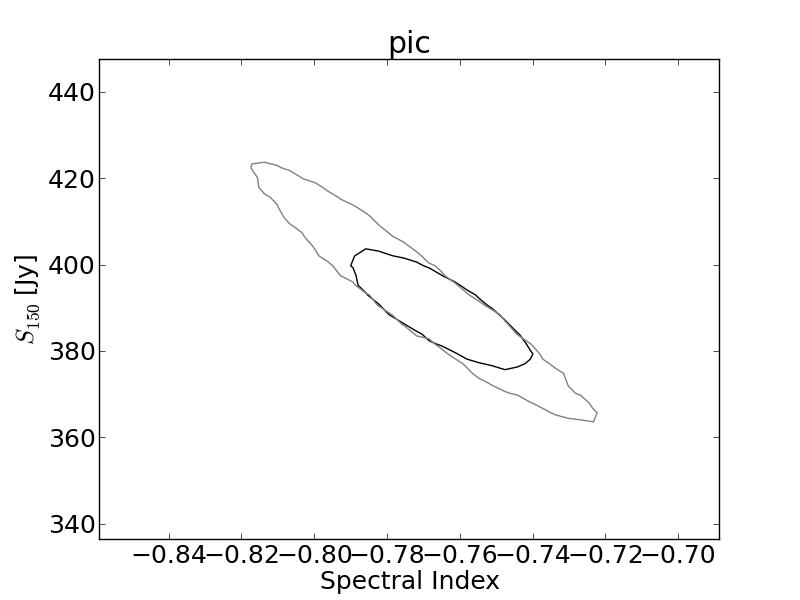
\includegraphics[width=0.49\textwidth]{plots/pic_SI_MCMC.png}
\caption{
Using new PAPER results to constrain the spectrum of Pictor A.  On the left,
the PAPER Pictor A spectrum with 2$\sigma$ error bars (x) and  MCMC fits (grey
cloud). Inset allows comparison between the 10MHz averaged points with the
403kHz points (grey). The oscillations in the PAPER spectrum are residual side
lobe contamination from other sources and are well represented by the error
bars.  The most reliable prior measurements (dots) are those by
\cite{Wills:1975p9314} at 580MHz and 635MHz \citep{Perley:1997p9312}. The rest
are from with Culgoora \cite{Slee:1995p7541} or Parkes
\cite{Otrupcek:1991p8780} and have been set to the (extrapolated)
\citet{Baars:1977p9678} scale by  \cite{Kuehr:1981p9628}. A sub-sample of MCMC
fits are shown in blue. On the right, the grey contour indicates the 76\%
confidence interval for 150MHz flux and spectral index given the prior data.
Black folds in the PAPER data.
} \label{fig:pic_spectrum}
\end{figure*}

%%calibrators
%%2250-412_2331-416_0043-424
%\begin{figure*}[htbp]
%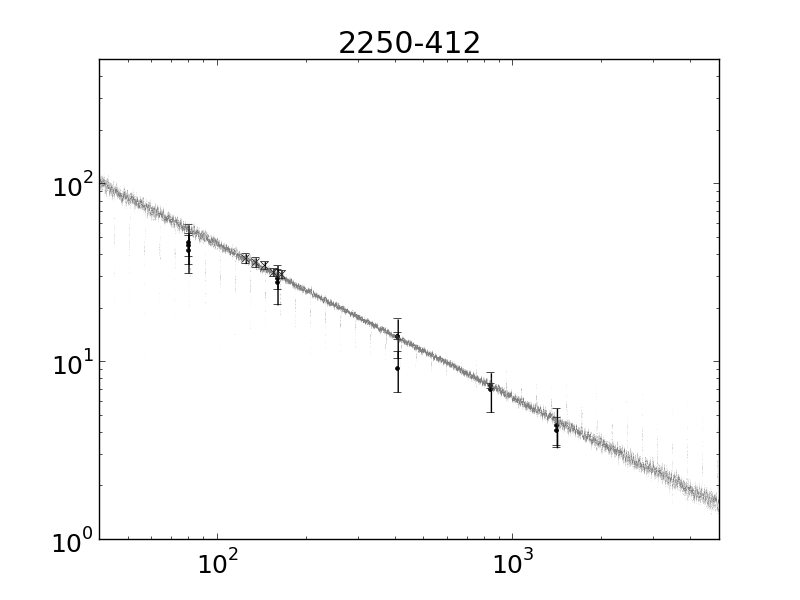
\includegraphics[width=0.2\textwidth]{plots/2250-412_calfit.png}
%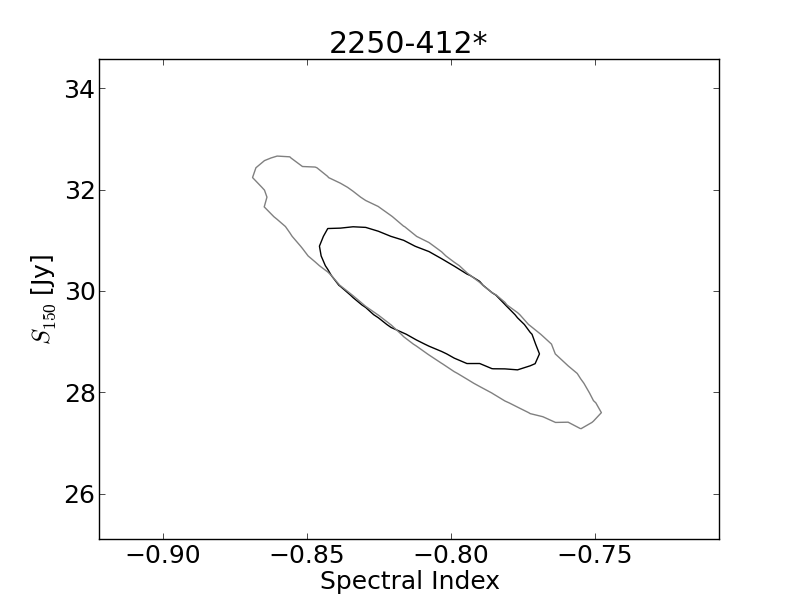
\includegraphics[width=0.2\textwidth]{plots/2250-412_SI_MCMC.png}
%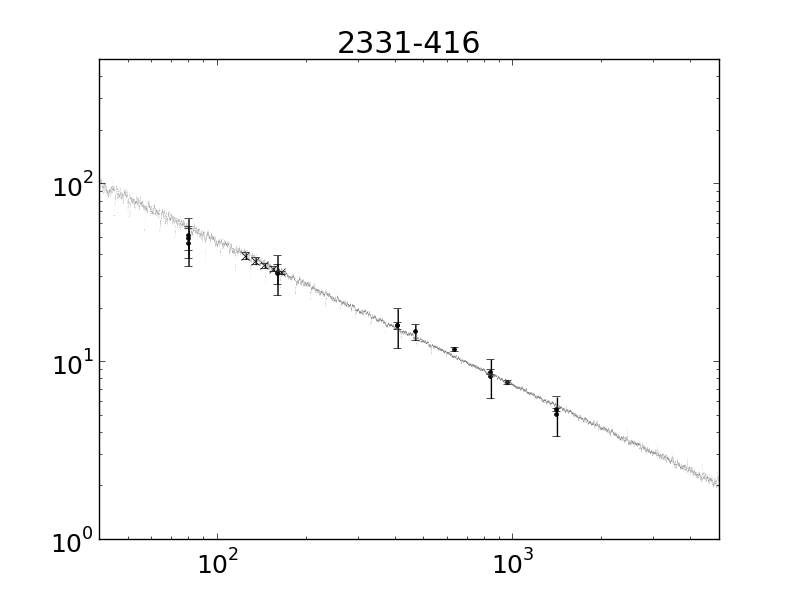
\includegraphics[width=0.2\textwidth]{plots/2331-416_calfit.png}
%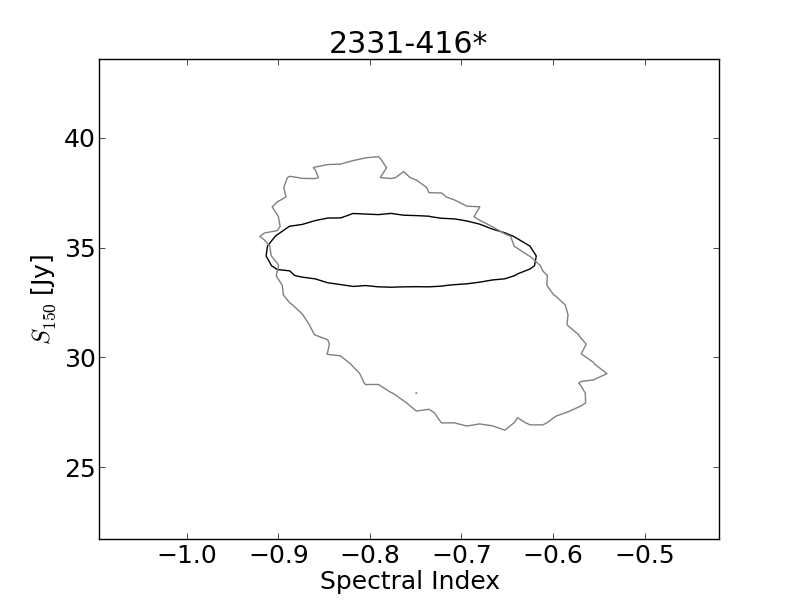
\includegraphics[width=0.2\textwidth]{plots/2331-416_SI_MCMC.png}\\
%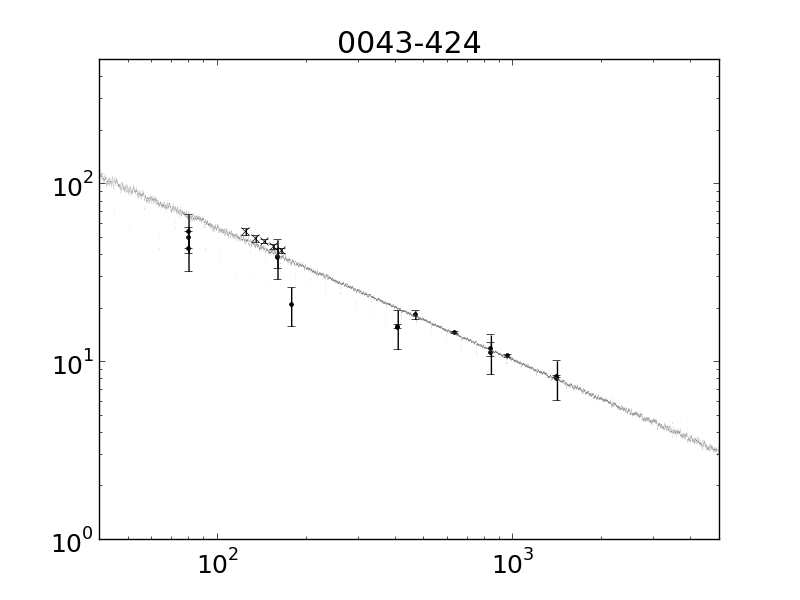
\includegraphics[width=0.2\textwidth]{plots/0043-424_calfit.png}
%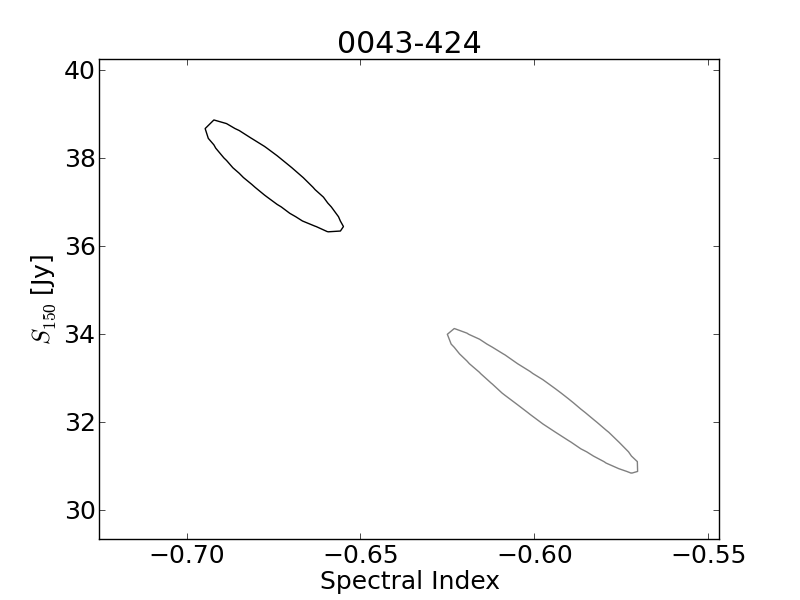
\includegraphics[width=0.2\textwidth]{plots/0043-424_SI_MCMC.png}
%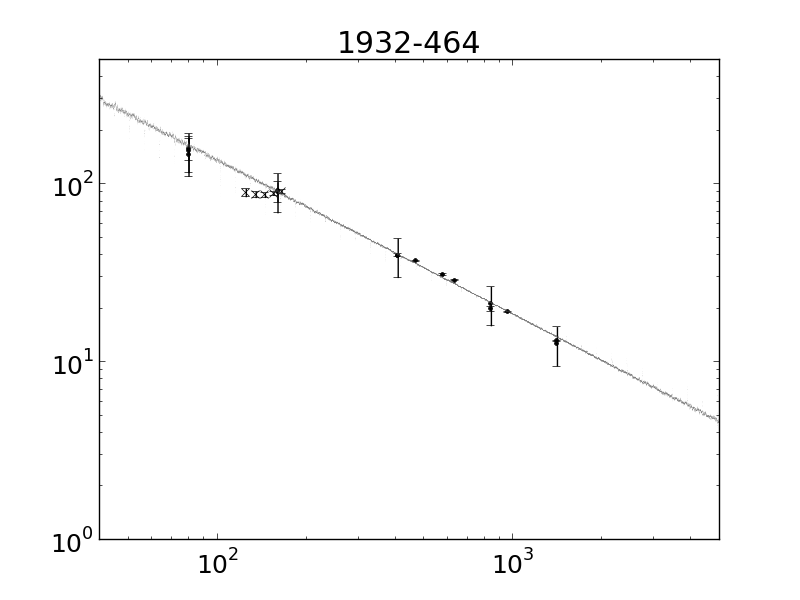
\includegraphics[width=0.2\textwidth]{plots/1932-464_calfit.png}
%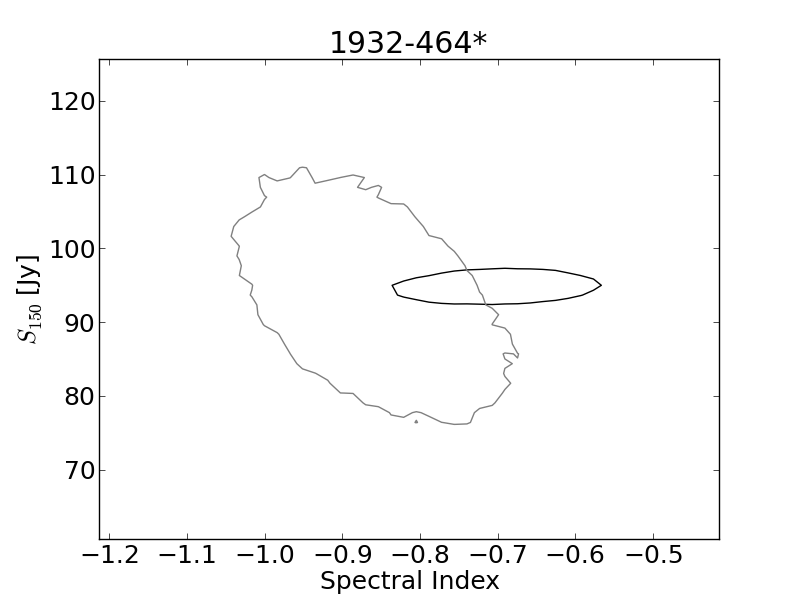
\includegraphics[width=0.2\textwidth]{plots/1932-464_SI_MCMC.png}
%
%\caption{Sources used to calculate the flux scale. Catalog data for the three sources are used to simultaneously fit a 
%single spectral index gain model for each source (grey contours) and a single PAPER gain parameter  .\label{fig:cals} }
%
%\end{figure*}
%add calibrator



\section*{Acknowledgements}

The PAPER project is supported by the National Science Foundation (awards
0804508, 1129258, and 1125558), and a generous grant from the Mt. Cuba
Astronomical Association.

This work makes use of ]the ``MCMC Hammer" emcee python library \citep[
\url{http://danfm.ca/emcee/}]{ForemanMackey:2012p8684}  and the NASA/IPAC
Extragalactic Database (NED) which is operated by the Jet Propulsion
Laboratory, California Institute of Technology, under contract with the
National Aeronautics and Space Administration.

\section*{Appendix: Model Fitting}
% XXX this should be in main body, not an appendix

In this paper we estimate spectral model parameters and flux calibration in a
Bayesian way by calculating and marginalizing the posterior probability of the
data, past and present, given a spectral and instrumental model.   This method
offers improved repeatability by specifying a single objective function that
represents the quality of the model fit and naturally defines the errors on the
parameters \citep{Hogg:2010p8759}.   See  \citet{Mackay:2003p9717}  or
\citet{Sivia:2006p9736} for more on Bayesian analysis methods and an excellent
astrophysical example by \cite{Press:1997p9783}.

In general an experiment measures data $D$ and given some model of the
statistics of the measurement one usually assigns an error bar defining the
probability of getting that data, given a model $M$.  Given all the new data,
and prior data, there will be a new optimal set of model parameters $M$ with
associated error bars.  In general, these error bars are a parameterization of
a probability distribution function.  The pdf associated with the data often
called the likelihood ($\mathcal{L}$), while the one corresponding the model
error bars is the {\em posterior probability distribution}, $\Prob(M|D)$. They
are related

\[
\Prob(M|D) = \frac{\mathcal{L}(D|M) \Prob(M)}{\Prob(D)}
\] 
by the factor $\frac{\Prob(M)}{\Prob(D)}$, the prior probability of the model
$M$ (given past experiments) over the normalization factor, integrating over
all models.  In general the posterior pdf depends on both the known relation
between the model parameters and as well as correlations hidden within the
data.  

Direct calculation of the posterior is difficult, particularly the
normalization factor, however there is a simple procedure for drawing samples
from the posterior. In this paper we use a Markov Chain Monte Carlo sampler.
Given any current location in parameter space, this algorithm draws a new set
of parameters and computes the relative likelihood increase. If the probability
difference is larger than a number drawn randomly from the set $(0:1]$, the
jump is accepted ---a Metropolis-Hastings step. In the limit of an infinity of
such steps, this process has been shown to converge on the true posterior
distribution.  In practice it is run for a large number of steps until things
appear to stabilize. The best fit model is the median of all the sampled
parameter sets, while the volume containing a well defined fraction of samples
sets the confidence limits.  The oft quoted ``1$\sigma$" probability level
corresponding to a gaussian distribution contains 65\% of the samples. In
practice the contours are not gaussian. Here we choose a slightly more
conservative probability level of 76\% 

In \S \ref{sec:fits} we fit a spectral power law to catalog values by sampling
a (log) likelihood which assumes Gaussian measurement errors

\[
\logL = \sum_\nu{\frac{\left(S_\nu - S150\left(\frac{\nu}{150}\right)^\alpha\right)^2}{\Delta \textrm{SPAPER}_\nu}} \label{eq:catlogL}
\]

We estimate the confidence interval of the resulting parameters as the boundary
enclosing 76\% of the samples. In the catalog we report both the upper and
lower of these values for both parameters and plot the 2D contour to show the
correlation of the two parameters. Many of these contours, the grey curves in
Fig. \ref{fig:SI_contour_1}, are classic banana plots, displaying a non-linear
correlation between the parameters.    In most cases the single contour
adequately describes 2D posterior distribution.

\begin{figure}[htbp]
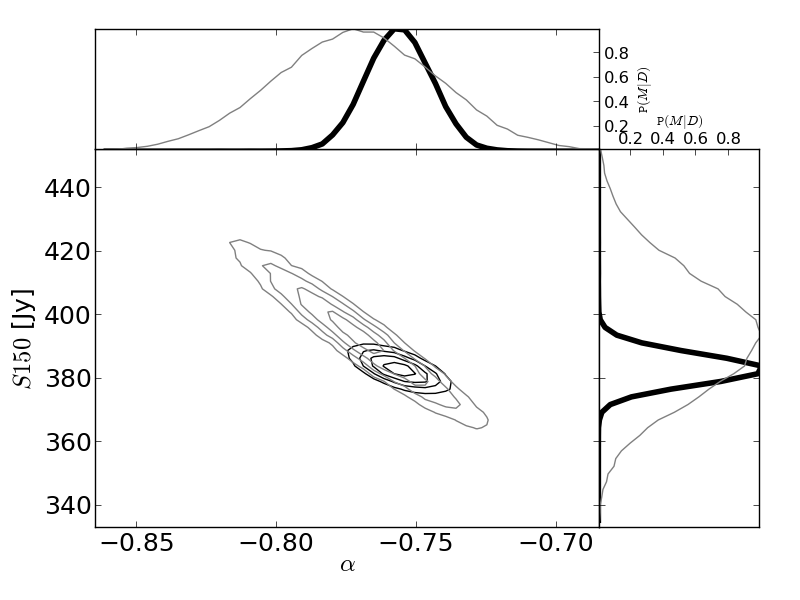
\includegraphics[width=0.49\textwidth]{plots/pic_trace_hist.png}
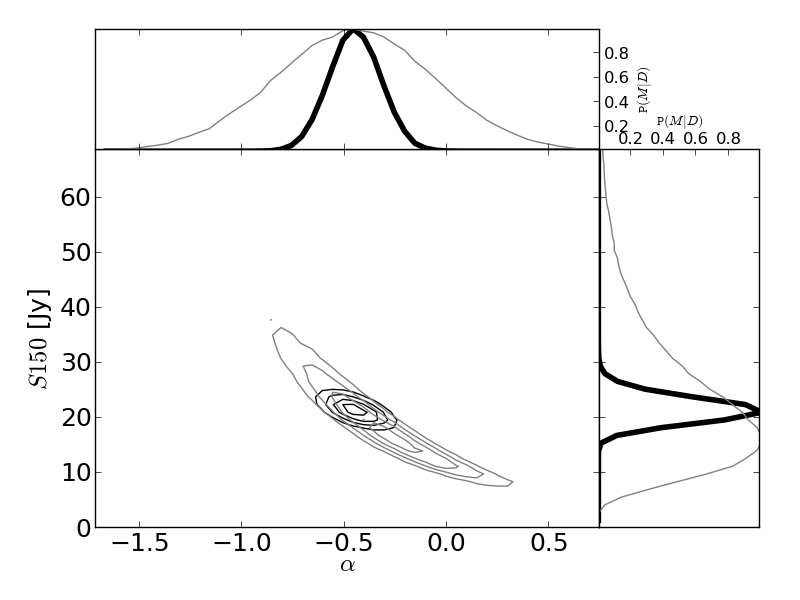
\includegraphics[width=0.49\textwidth]{plots/1556-466_trace_hist.png}
\caption{
A more detailed view of the posterior probability distribution. On the left
Pictor A, on the right 1556-466. Confidence contours range from 0.2 to 0.8.
Compare with the contours for this source shown in Fig. \ref{fig:SI_contour_3}.
As above, grey for  the fit to catalog data, black for joint catalog and PAPER
fit.
}
\end{figure}


A single overall flux scale is computed in a similar way. However, here we add
a single extra gain factor $g$ multiplying all PAPER measurements, and sum over
several sources.

\begin{align}
\log\mathcal{L}_s &= \sum_{\nu}\frac{ (S_\textrm{cat}^{\nu}  - S_{150}  \left(\frac{\nu}{150}\right)^\alpha)^2}{2(\Delta S_\textrm{cat}^\nu)^2} +
\frac{ (g*S_\PAPER^{\nu}  - S_{150}\left(\frac{\nu}{150}\right)^\alpha)^2}{2(\Delta S_\PAPER^\nu)^2}\\
\log\mathcal{L} &= \sum_{s} \log\mathcal{L}_s
\end{align}
Another nice feature of the MCMC sampler is that each parameter sample is fully
covariant with the others. To marginalize over the fitted flux and spectral
index parameters and compute confidence limits on the gain parameter, we simply
ignore them.


\begin{figure*}[htbp]
\begin{center}
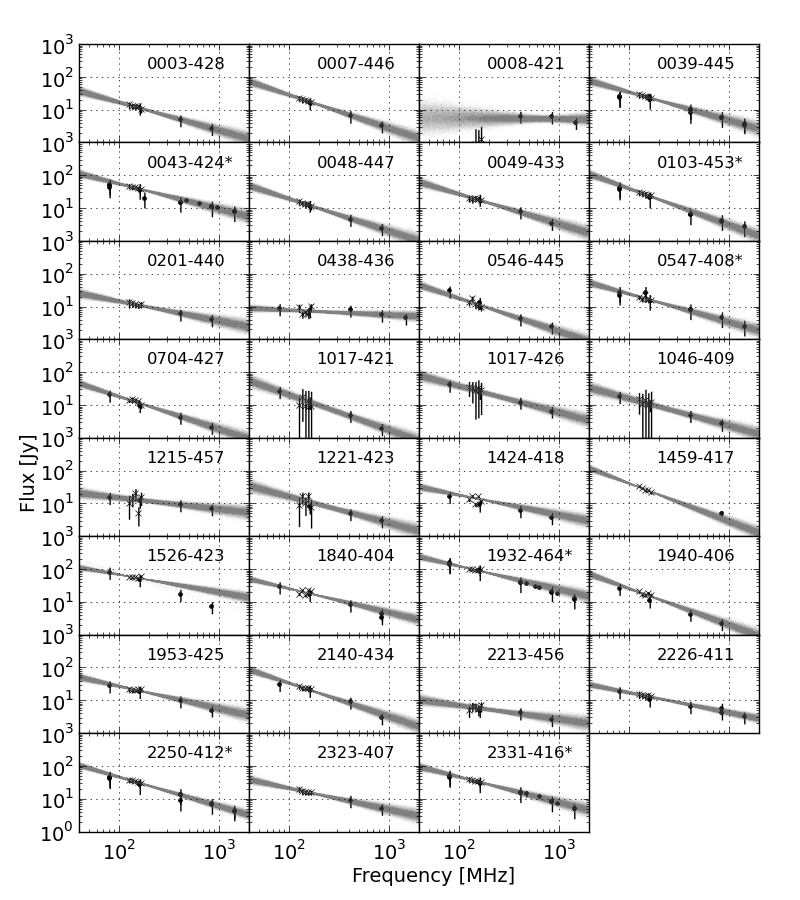
\includegraphics[width=0.9\textwidth]{plots/srcfig_1.png}
\end{center}
\caption{
PAPER spectra of 16 sources compared against existing data out of
\cite{Vollmer:2010p6422} between 40MHz and 2GHz, otherwise as described in
Figure \ref{fig:pic_spectrum}.\label{fig:srcs1}. Sources used to bootstrap the
flux calibration are noted with a *.
}
\end{figure*}

\begin{figure*}[htbp]
\begin{center}
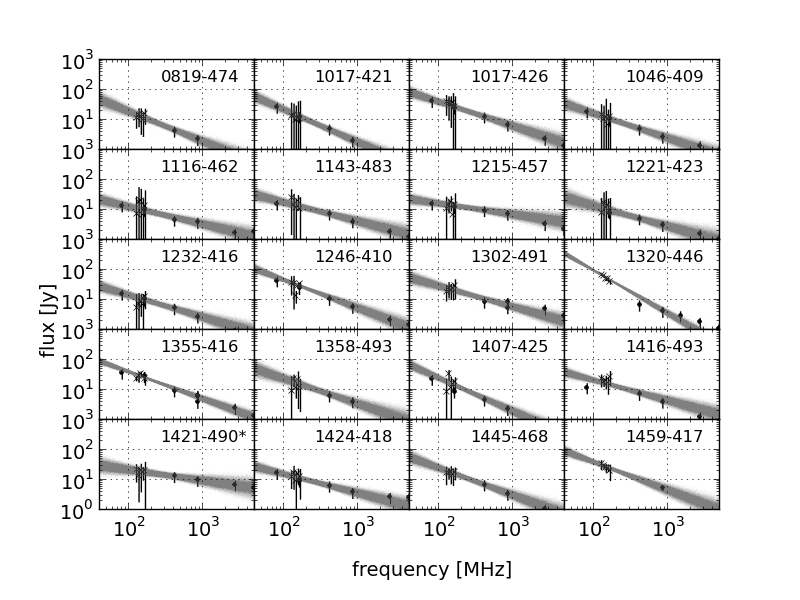
\includegraphics[width=0.9\textwidth]{plots/srcfig_2.png}
\caption{
PAPER spectra of 16 sources compared against existing data out of
\cite{Vollmer:2010p6422} between 40MHz and 2GHz, otherwise as described in
Figure \ref{fig:pic_spectrum}.\label{fig:srcs2} Sources used to bootstrap the
flux calibration are noted with a *.
}
\end{center}
\end{figure*}

\begin{figure*}[htbp]
\begin{center}
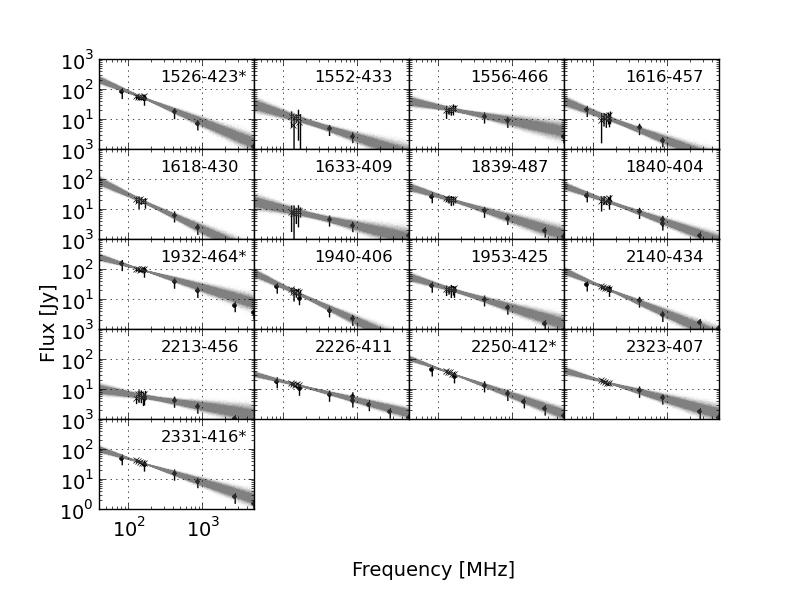
\includegraphics[width=0.9\textwidth]{plots/srcfig_3.png}
\caption{
PAPER spectra of 16 sources compared against existing data out of
\cite{Vollmer:2010p6422} between 40MHz and 2GHz, otherwise as described in
Figure \ref{fig:pic_spectrum}.\label{fig:srcs3} Sources used to bootstrap the
flux calibration are noted with a *.
}
\end{center}
\end{figure*}



%(PAPER_imaging)danny@keynes:plots$ python sort_SI_plots.py psa64_pic_stripe_perleycorr_SEDfits.txt
%BEGIN PASTE
%the best sources. High quality fit that improves on previous knowledge
\begin{figure*}[htbp]
\begin{center}
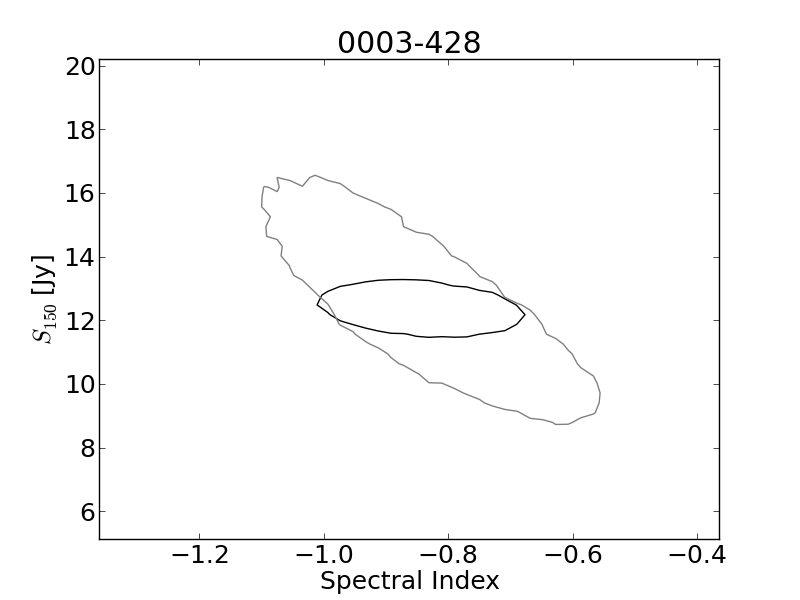
\includegraphics[width=2in]{plots/0003-428_SI_MCMC.png} %0.1064
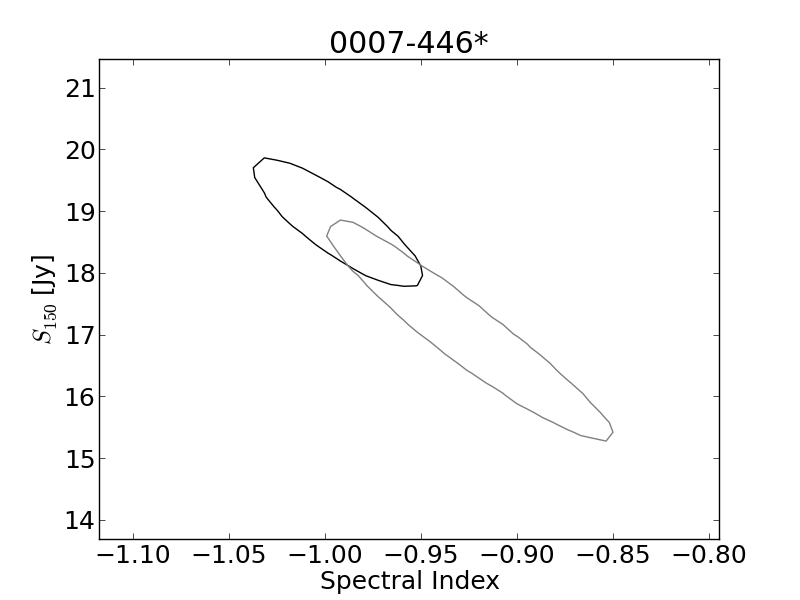
\includegraphics[width=2in]{plots/0007-446_SI_MCMC.png} %0.1851
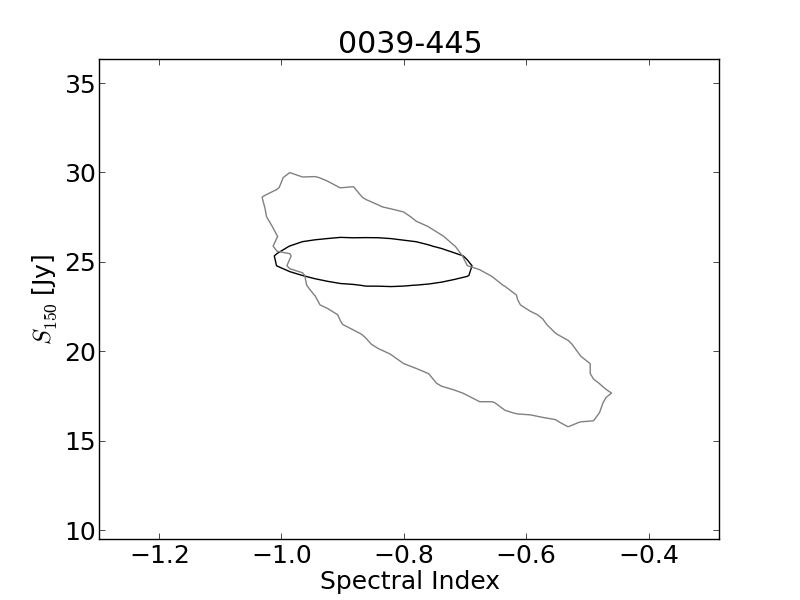
\includegraphics[width=2in]{plots/0039-445_SI_MCMC.png} %0.7325
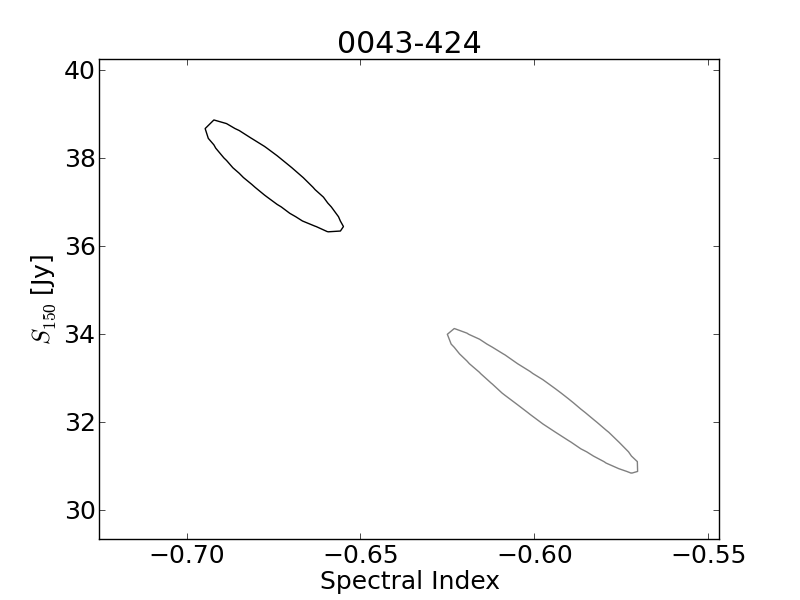
\includegraphics[width=2in]{plots/0043-424_SI_MCMC.png} %0.2527
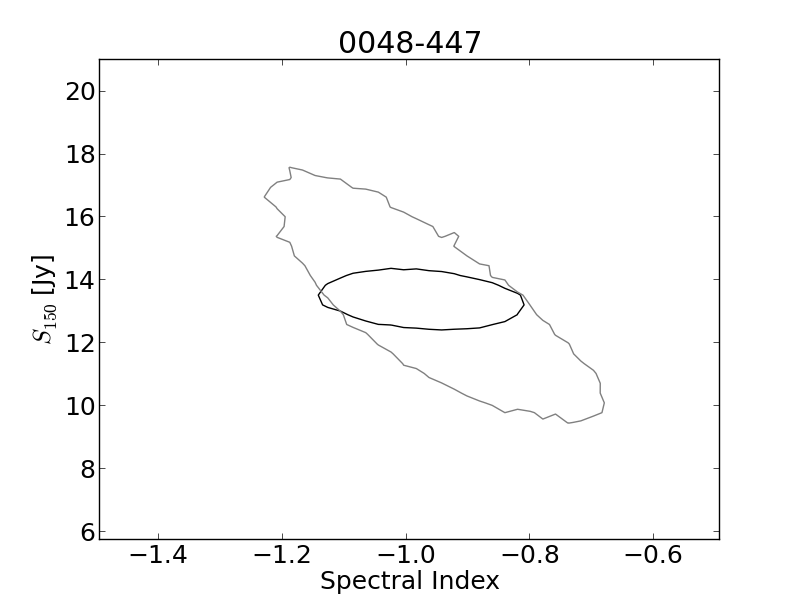
\includegraphics[width=2in]{plots/0048-447_SI_MCMC.png} %0.0596
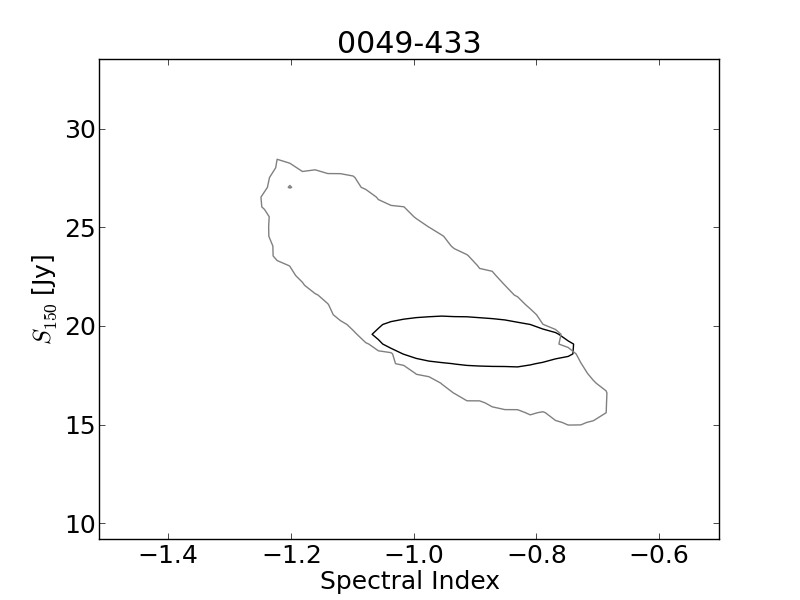
\includegraphics[width=2in]{plots/0049-433_SI_MCMC.png} %0.2988
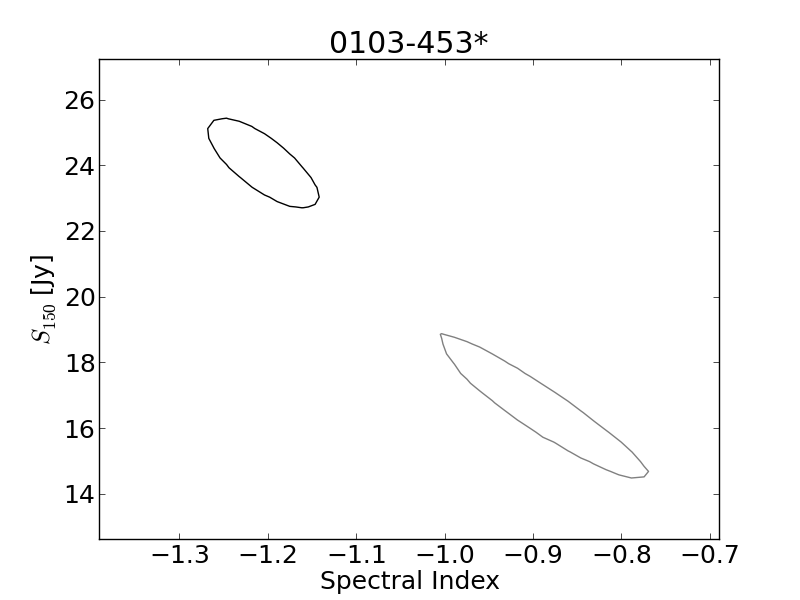
\includegraphics[width=2in]{plots/0103-453_SI_MCMC.png} %0.007
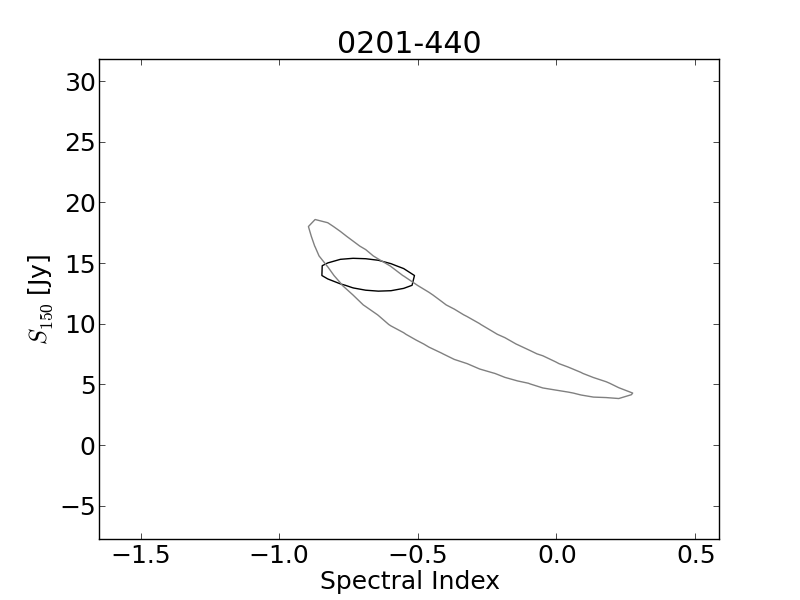
\includegraphics[width=2in]{plots/0201-440_SI_MCMC.png} %2.3481
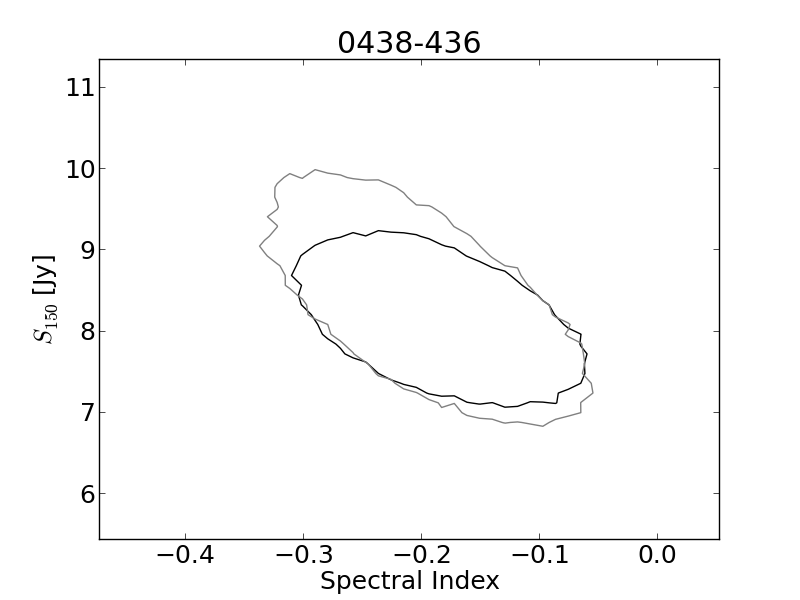
\includegraphics[width=2in]{plots/0438-436_SI_MCMC.png} %0.0595
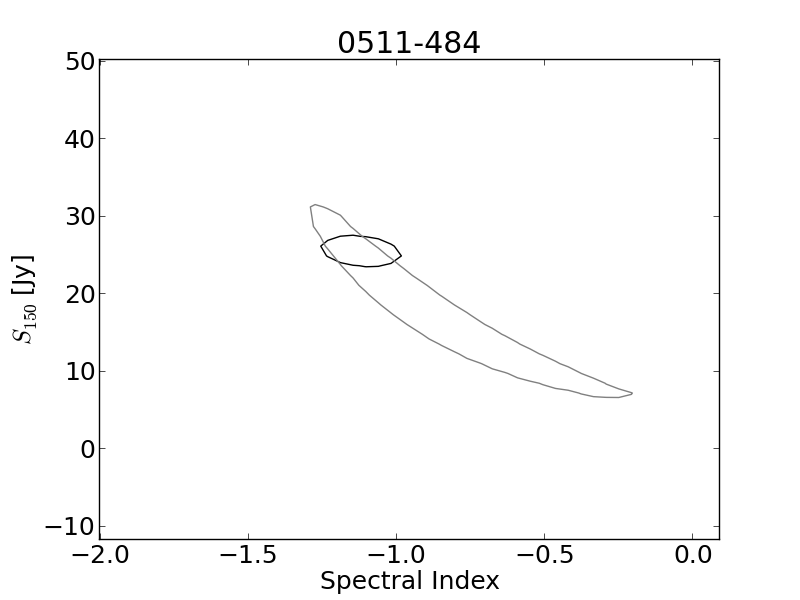
\includegraphics[width=2in]{plots/0511-484_SI_MCMC.png} %2.6709
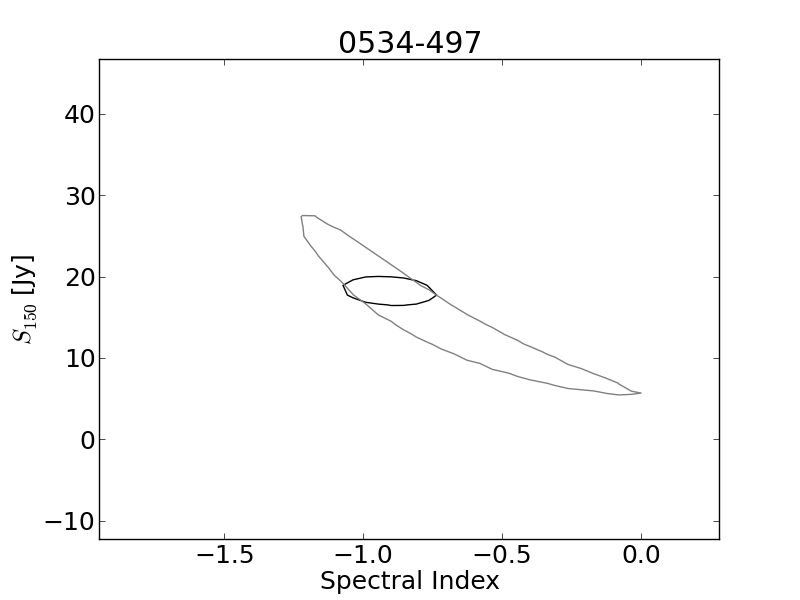
\includegraphics[width=2in]{plots/0534-497_SI_MCMC.png} %2.6256
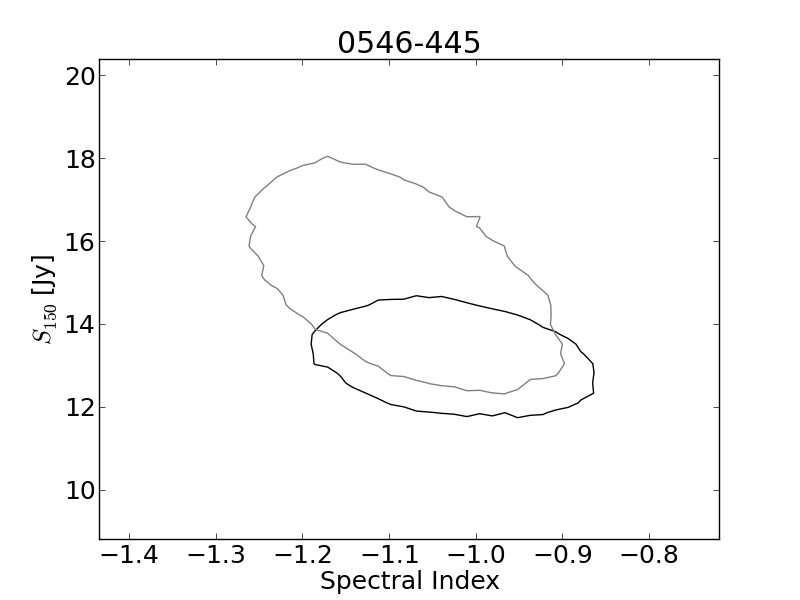
\includegraphics[width=2in]{plots/0546-445_SI_MCMC.png} %0.1024
\end{center}
\caption{Spectral model contours as described in Figure \ref{fig:pic_spectrum}. Sources marked with a
* were used to assess calibration error.
}\label{fig:SI_contour_1}
\end{figure*}
\clearpage
\begin{figure*}[htbp]2\begin{center}
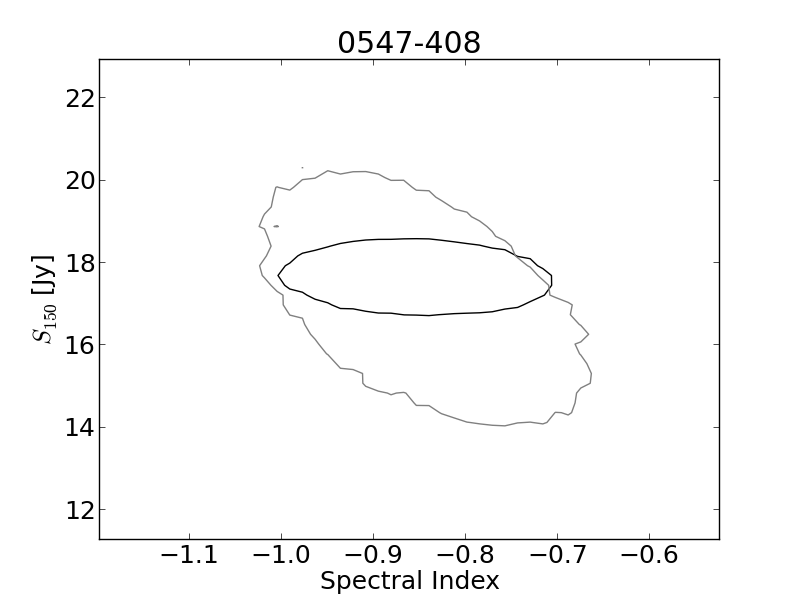
\includegraphics[width=2in]{plots/0547-408_SI_MCMC.png} %0.1044
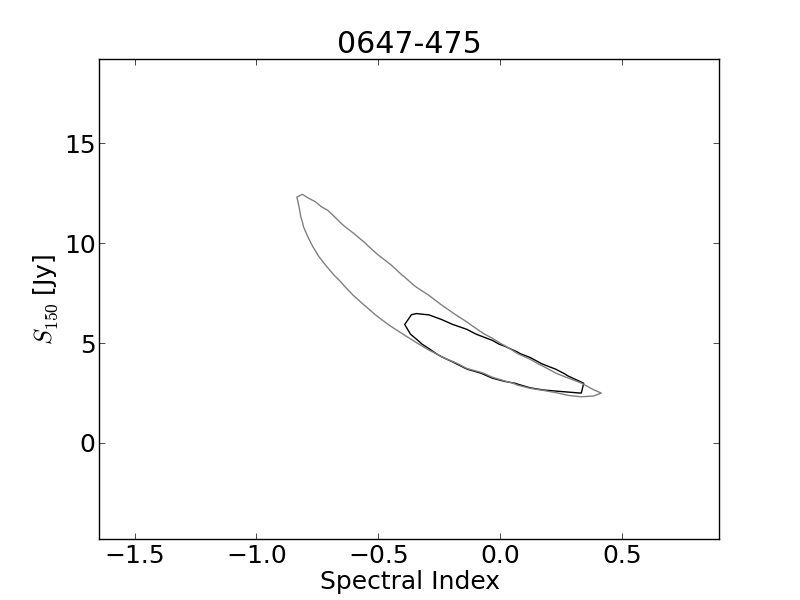
\includegraphics[width=2in]{plots/0647-475_SI_MCMC.png} %0.8893
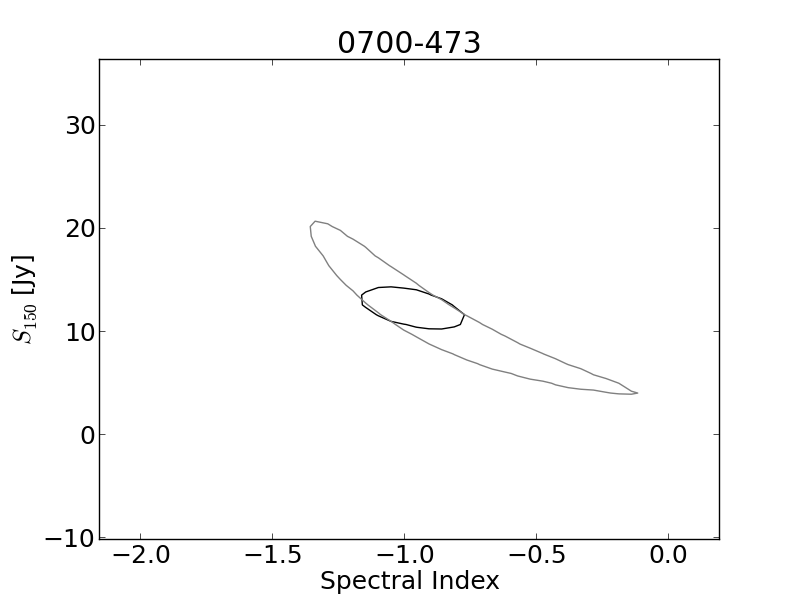
\includegraphics[width=2in]{plots/0700-473_SI_MCMC.png} %1.709
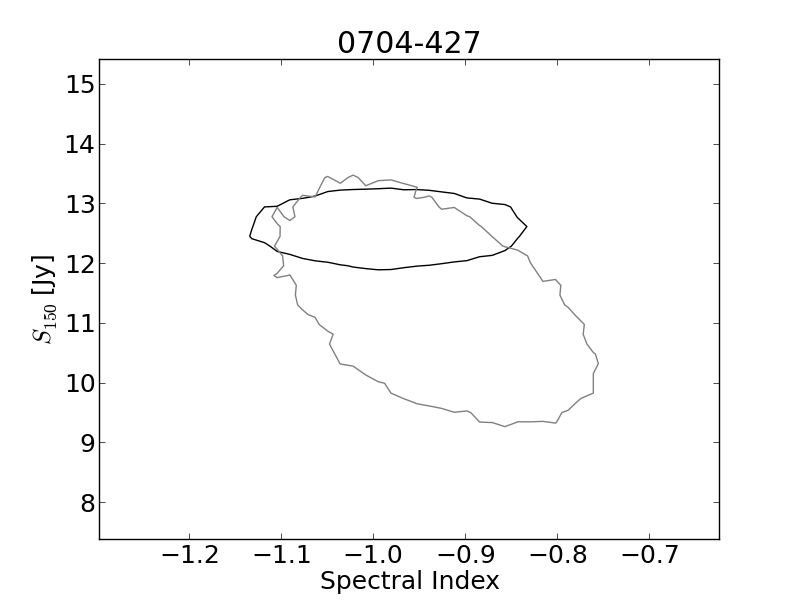
\includegraphics[width=2in]{plots/0704-427_SI_MCMC.png} %0.0824
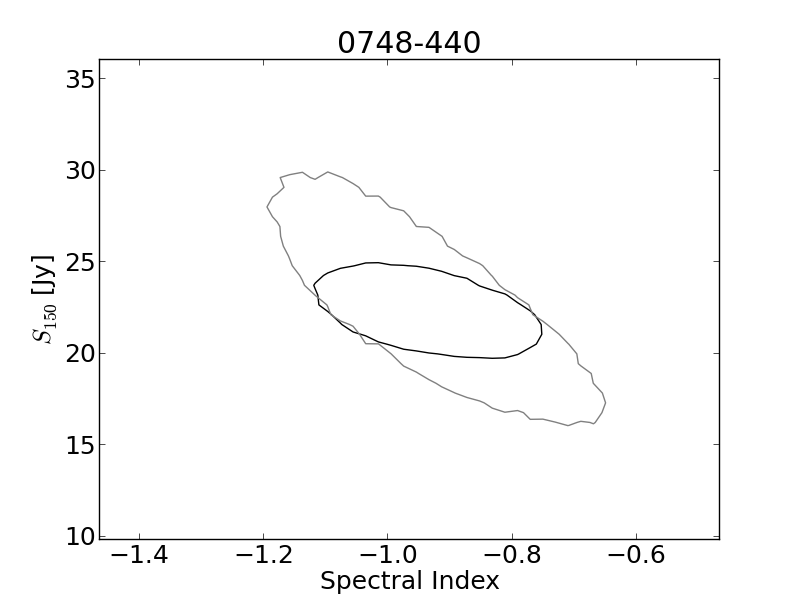
\includegraphics[width=2in]{plots/0748-440_SI_MCMC.png} %0.3377
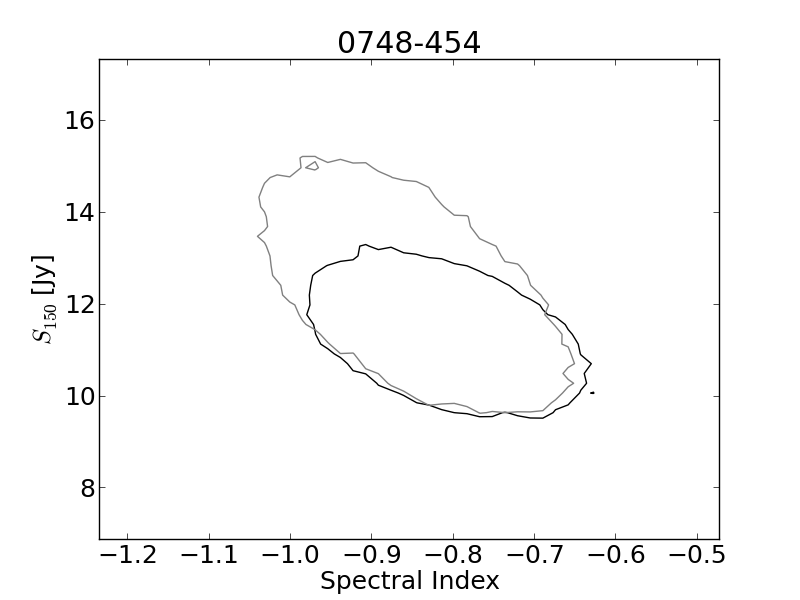
\includegraphics[width=2in]{plots/0748-454_SI_MCMC.png} %0.0699
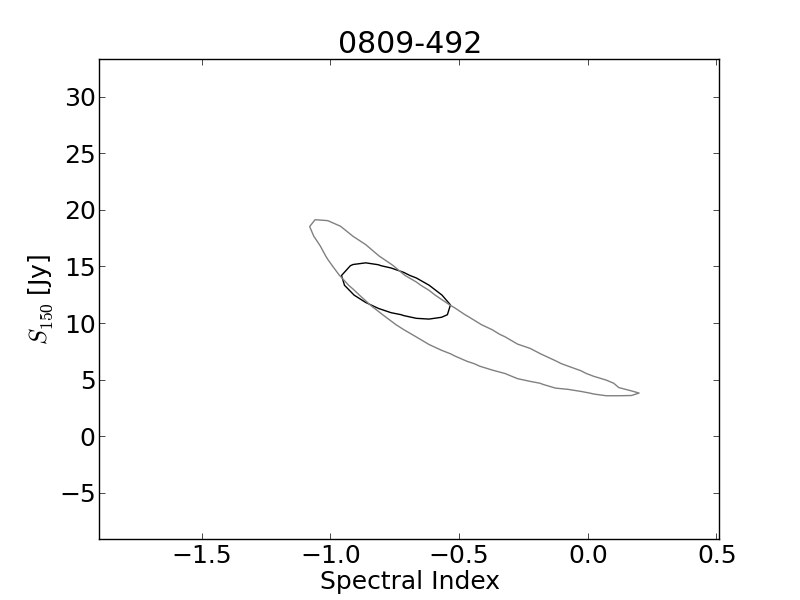
\includegraphics[width=2in]{plots/0809-492_SI_MCMC.png} %1.2296
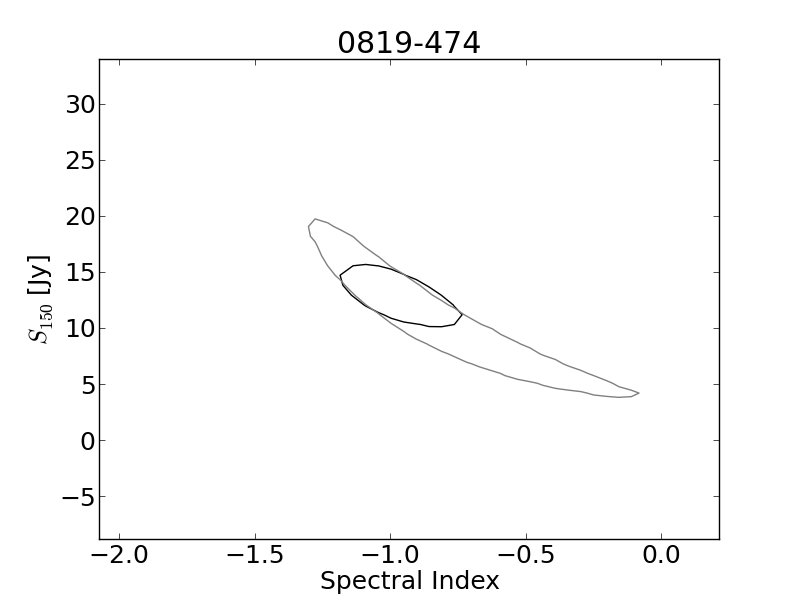
\includegraphics[width=2in]{plots/0819-474_SI_MCMC.png} %1.5069
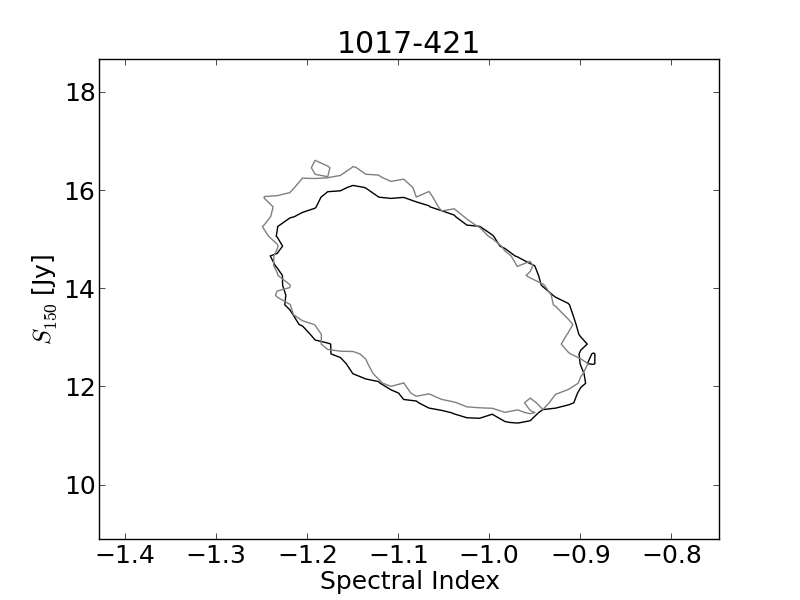
\includegraphics[width=2in]{plots/1017-421_SI_MCMC.png} %0.0031
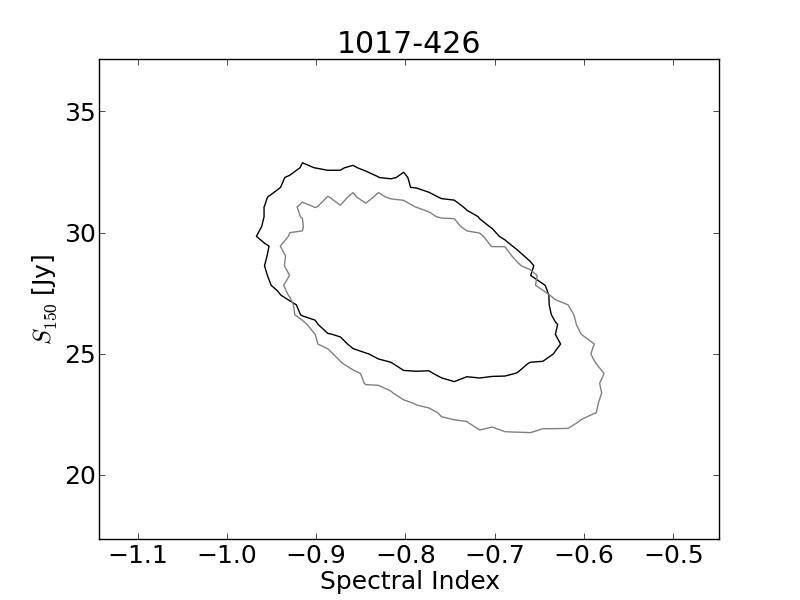
\includegraphics[width=2in]{plots/1017-426_SI_MCMC.png} %0.0455
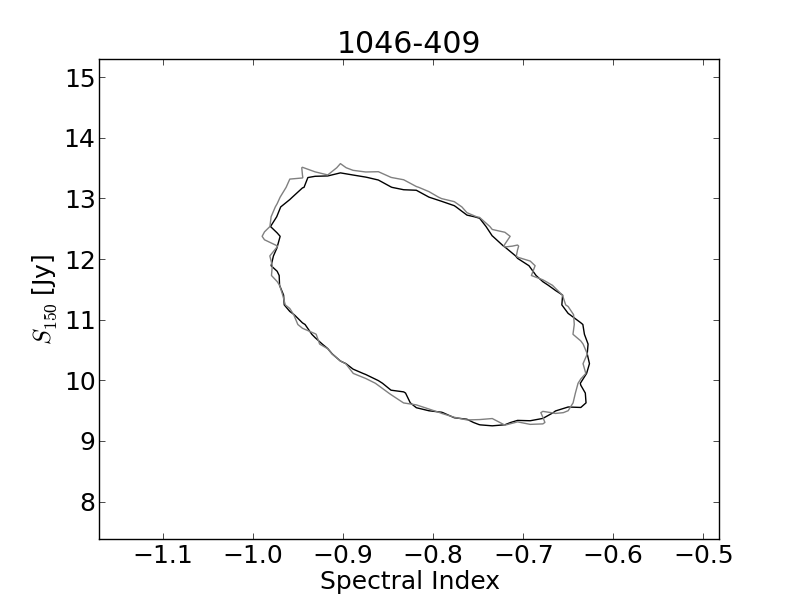
\includegraphics[width=2in]{plots/1046-409_SI_MCMC.png} %0.0055
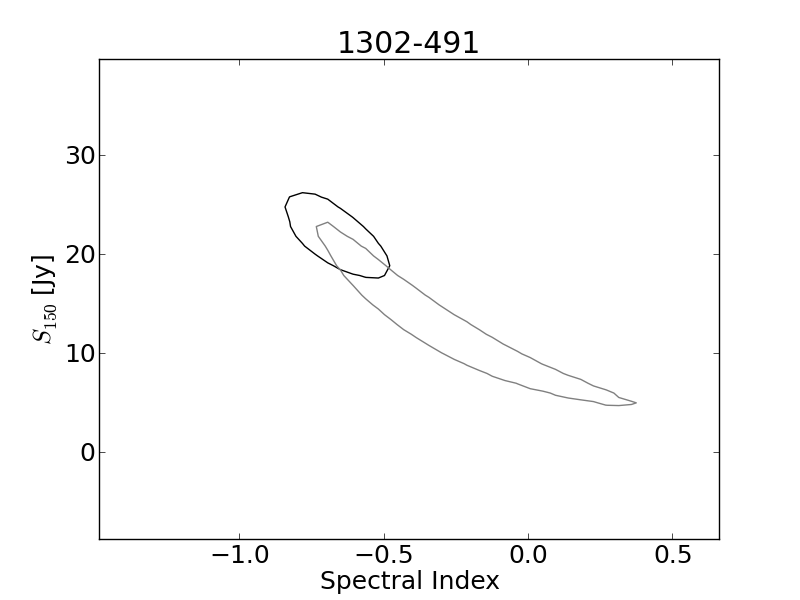
\includegraphics[width=2in]{plots/1302-491_SI_MCMC.png} %0.0592
\end{center}
\caption{Spectral model contours as described in Figure \ref{fig:pic_spectrum}. Sources marked with a
* were used to assess calibration error.
}\label{fig:SI_contour_2}
\end{figure*}
\clearpage
\begin{figure*}[htbp]2\begin{center}
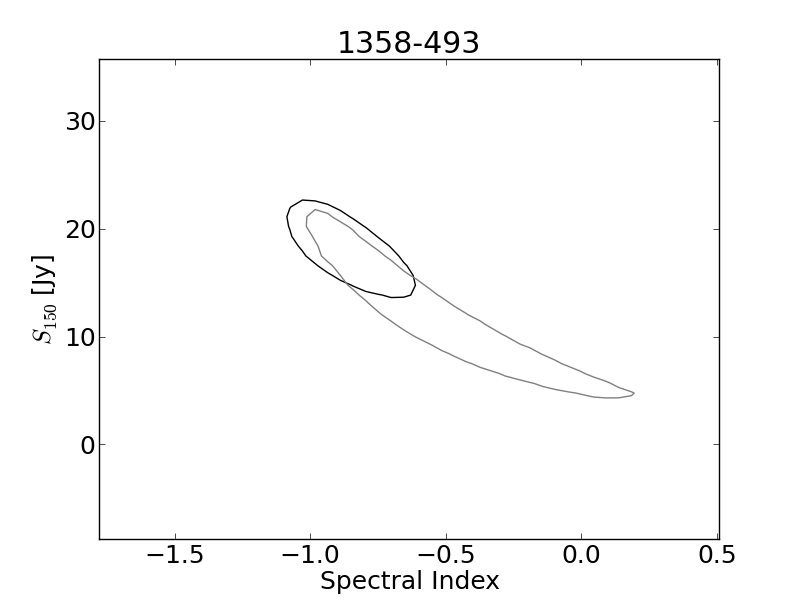
\includegraphics[width=2in]{plots/1358-493_SI_MCMC.png} %0.4795
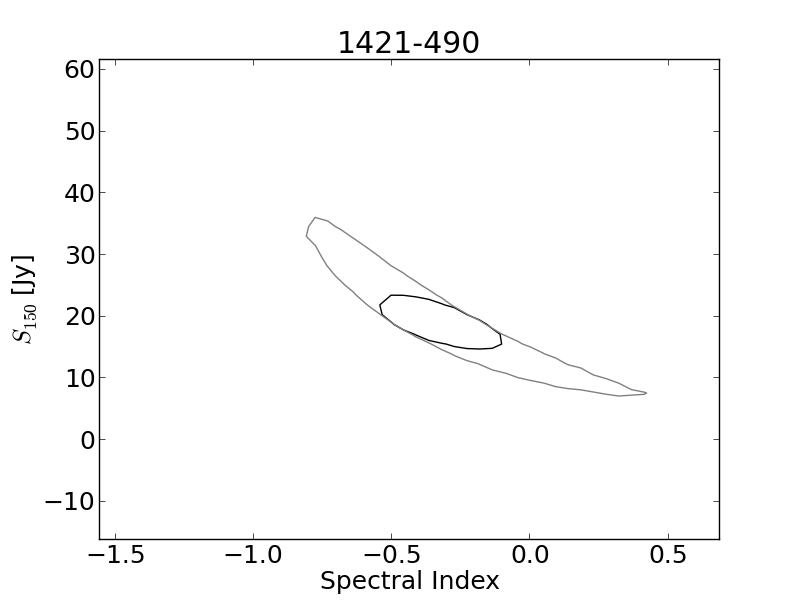
\includegraphics[width=2in]{plots/1421-490_SI_MCMC.png} %0.891
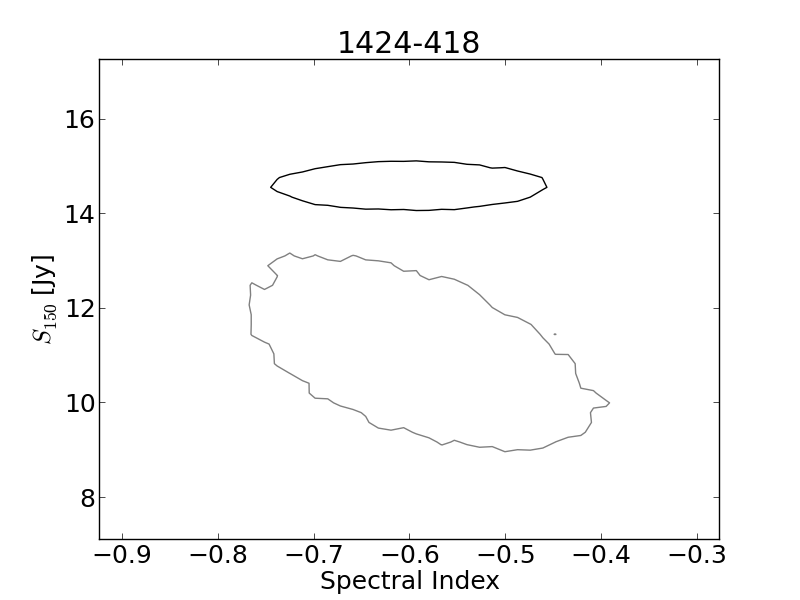
\includegraphics[width=2in]{plots/1424-418_SI_MCMC.png} %0.0056
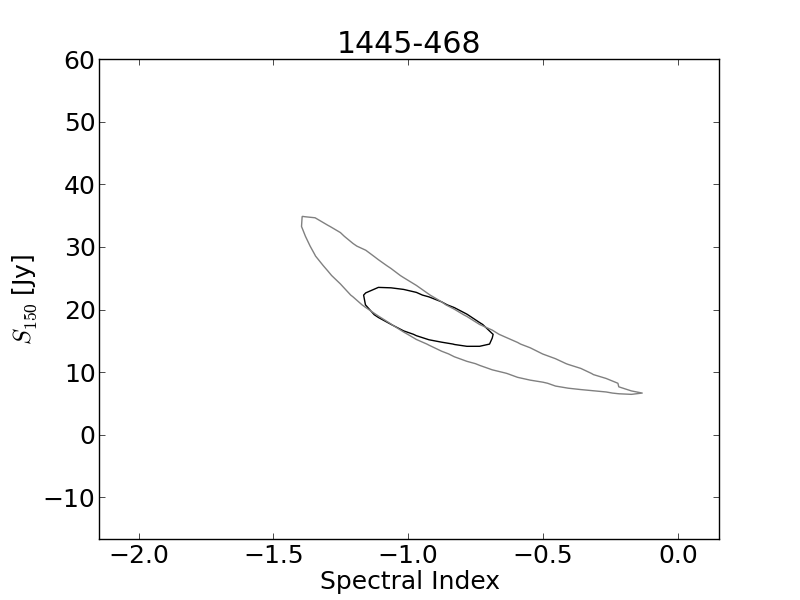
\includegraphics[width=2in]{plots/1445-468_SI_MCMC.png} %0.973
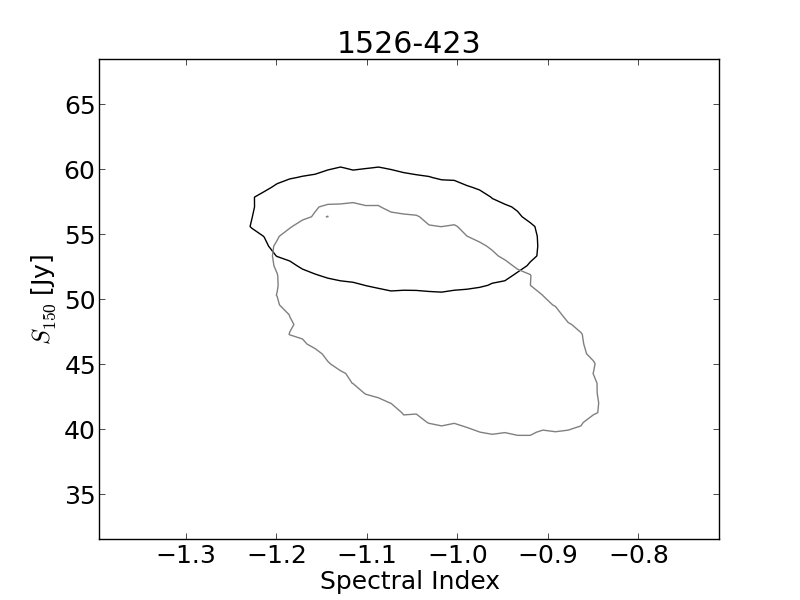
\includegraphics[width=2in]{plots/1526-423_SI_MCMC.png} %0.0961
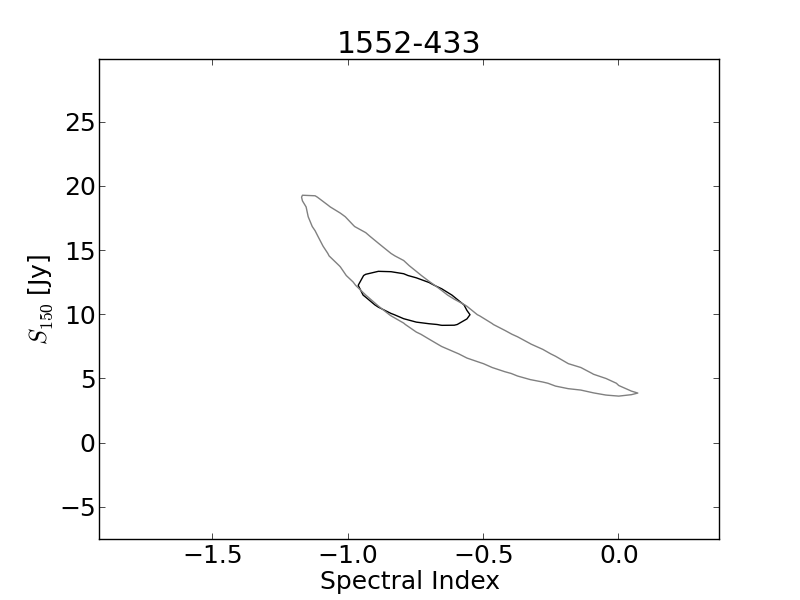
\includegraphics[width=2in]{plots/1552-433_SI_MCMC.png} %0.9684
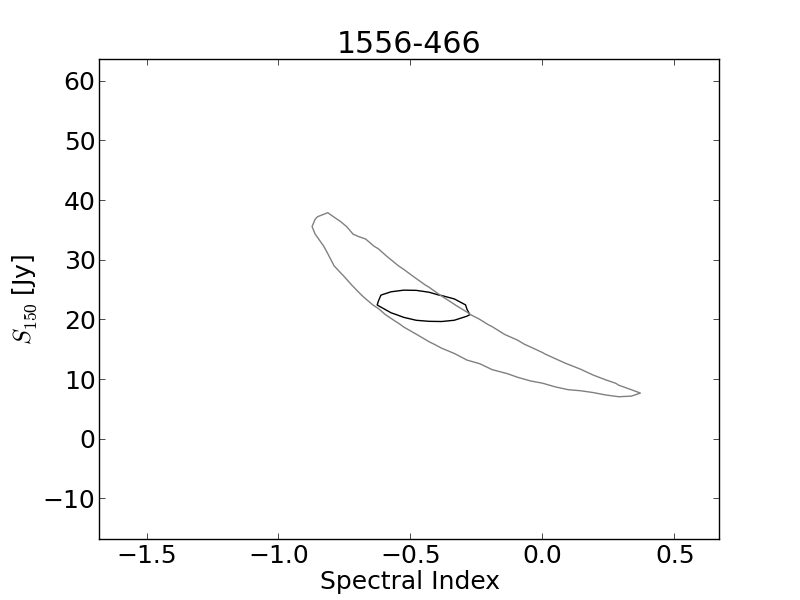
\includegraphics[width=2in]{plots/1556-466_SI_MCMC.png} %1.4713
\includegraphics[width=2in]{plots/1616-457_SI_MCMC.png} %0.0157
\includegraphics[width=2in]{plots/1618-430_SI_MCMC.png} %2.7782
\includegraphics[width=2in]{plots/1633-409_SI_MCMC.png} %0.2602
\includegraphics[width=2in]{plots/1839-487_SI_MCMC.png} %0.135
\includegraphics[width=2in]{plots/1840-404_SI_MCMC.png} %0.1159
\end{center}
\caption{Spectral model contours as described in Figure \ref{fig:pic_spectrum}. Sources marked with a
* were used to assess calibration error.
}\label{fig:SI_contour_3}
\end{figure*}
\clearpage
\begin{figure*}[htbp]2\begin{center}
\includegraphics[width=2in]{plots/1932-464_SI_MCMC.png} %0.0164
\includegraphics[width=2in]{plots/1940-406_SI_MCMC.png} %0.0524
\includegraphics[width=2in]{plots/1953-425_SI_MCMC.png} %0.0739
\includegraphics[width=2in]{plots/2140-434_SI_MCMC.png} %0.3123
\includegraphics[width=2in]{plots/2213-456_SI_MCMC.png} %0.1767
\includegraphics[width=2in]{plots/2226-411_SI_MCMC.png} %0.1166
\includegraphics[width=2in]{plots/2250-412_SI_MCMC.png} %0.2199
\includegraphics[width=2in]{plots/2323-407_SI_MCMC.png} %6.9237
\includegraphics[width=2in]{plots/2331-416_SI_MCMC.png} %0.2179
\end{center}
\caption{fits of the next 16 sources, as described in Figure \ref{fig:SI_contour_1}. Sources marked with a
* were used to assess calibration error.
}\label{fig:SI_contour_4}
\end{figure*}
%BEGIN PASTE
\begin{figure*}[htbp]
\begin{center}
%ok fit, but doesn't agree with past data, or actually increases model uncertainty
%contour length limit =  209.039667221
%Poor improvement:  1116-462 8.66,9.97,11.27 -0.72,-0.59,-0.47 8.56,9.82,11.15 -0.71,-0.58,-0.46 0.22 0.23 -0 0.6 -0.0018 164.0
\includegraphics[width=2in]{plots/1116-462_SI_MCMC.png} %-0.0018
%Poor improvement:  1143-483 13.47,15.46,17.58 -0.83,-0.7,-0.57 9.91,11.65,13.51 -0.7,-0.56,-0.44 0.34 0.37 -0.03 0.21 -0.0064 122.0
\includegraphics[width=2in]{plots/1143-483_SI_MCMC.png} %-0.0064
%Poor improvement:  1215-457 15.08,16.94,18.88 -0.59,-0.47,-0.36 11.28,12.93,14.57 -0.46,-0.33,-0.21 0.36 0.39 -0.03 0.15 -0.0042 122.0
\includegraphics[width=2in]{plots/1215-457_SI_MCMC.png} %-0.0042
%Poor improvement:  1221-423 9.46,11.52,13.87 -0.96,-0.78,-0.61 6.77,8.6,10.49 -0.78,-0.57,-0.39 0.45 0.53 -0.08 0.27 -0.022 116.0
\includegraphics[width=2in]{plots/1221-423_SI_MCMC.png} %-0.022
%Poor improvement:  1232-416 9.42,10.83,12.3 -0.88,-0.75,-0.63 9.2,10.57,11.96 -0.88,-0.74,-0.62 0.22 0.22 -0 0.57 -0.002 164.0
\includegraphics[width=2in]{plots/1232-416_SI_MCMC.png} %-0.002
%Poor improvement:  1407-425 13.6,15.19,16.86 -1.21,-1.09,-0.98 9.91,11.35,12.85 -1.07,-0.94,-0.82 0.36 0.41 -0.05 0.11 -0.0059 128.0
\includegraphics[width=2in]{plots/1407-425_SI_MCMC.png} %-0.0059
\end{center}
\caption{fits of the worst sources. Contours as described in Figure \ref{fig:SI_contour_1}. The fit either disagrees
with past data or does not offer any improvement (improvement index $\le 0$). All are near
the galactic plane and are likely dominated by sidelobes.
}\label{fig:SI_contour_bad}
\end{figure*}

\begin{figure*}[htbp]
\begin{center}
%zero overlap
\includegraphics[width=2in]{plots/1246-410_SI_MCMC.png} %-0
\includegraphics[width=2in]{plots/1320-446_SI_MCMC.png} %0.0
\includegraphics[width=2in]{plots/1355-416_SI_MCMC.png} %0.0
\includegraphics[width=2in]{plots/1416-493_SI_MCMC.png} %-0
\includegraphics[width=2in]{plots/1459-417_SI_MCMC.png} %0
\includegraphics[width=2in]{plots/cen_SI_MCMC.png} %0.0
\end{center}
\caption{
These sources offer results at odds with previous measurements. These have
small enough error bars to require a deviation from spectral index fit
suggested by prior catalog measurements. All are near Centaurus A (see Figure
\ref{fig:error_map}), a very bright, extended source, and are likely evidence
for side lobe contamination.  Side lobes from distant sources manifest as
ripples in the spectrum, increasing the error bars (e.g. the sources listed in
Figure \ref{fig:SI_contour_bad}). However, the sources shown here are close
enough to Centaurus A that the side-lobe oscillates on scales longer than 10MHz
and does not fall into the rms, but rather into the mean. Thus these few points
have anomalously high fluxes and small error bars. 
} \label{fig:SI_contour_new}
\end{figure*}


%END PASTE



\begin{figure*}
\includegraphics[width=\textwidth]{plots/psa64_pic_strip_positions_annotated_cropped.png}
\caption{
A map of the radio sky centered on the south pole
\citep{deOliveiraCosta:2008p2242}.  x's mark measured locations and have size
scaled by agreement with prior data (inverse ``improvement index", see
\S\ref{sec:fits}). Black dots indicate sources with $\le0$ improvement score.
For these the fit quality decreases with addition of PAPER data or the model
revision disagrees completely with the prior estimate due to side lobes or
spectral curvature.  We estimate that   \label{fig:error_map}
}
\end{figure*}


%TODO catalog format, table for data points and a table for fit results


\begin{deluxetable}{lllllllllllll}
\tablecolumns{13}
\tablecaption{PAPER spectra for 59 MRC sources. Full table available online}
\tablehead{
\colhead{Name} &
\colhead{\parbox[c][3em]{2em}{Ra \unit{deg}}} & 
\colhead{\parbox[c][2em]{2em}{Dec \unit{deg}}} &
\colhead{\parbox[c][2em]{2em}{S125 \unit{Jy}}} &
\colhead{\parbox[c][2em]{2em}{rms \unit{Jy}}} &
\colhead{\parbox[c][2em]{2em}{S135 \unit{Jy}}} &
\colhead{\parbox[c][2em]{2em}{rms \unit{Jy}}} &
\colhead{\parbox[c][2em]{2em}{S145 \unit{Jy}}} &
\colhead{\parbox[c][2em]{2em}{rms \unit{Jy}}} &
\colhead{\parbox[c][2em]{2em}{S155 \unit{Jy}}} &
\colhead{\parbox[c][2em]{2em}{rms \unit{Jy}}} &
\colhead{\parbox[c][2em]{2em}{S165 \unit{Jy}}} &
\colhead{\parbox[c][2em]{2em}{rms \unit{Jy}}}
}
\startdata
Pictor A&	80.1&	-45.79&	459.23&	30.2&	416.59&	28.3&	397.17&	21.8&	375.14&	18.5&	359.72&	17.1 \\
0003-428&	1.67&	-42.5&	14.98&	2.0&	13.45&	1.2&	13.02&	1.8&	12.9&	1.6&	10.42&	1.2 \\
0007-446&	2.79&	-44.31&	23.51&	2.5&	21.18&	2.4&	20.24&	1.5&	18.74&	1.5&	17.61&	1.8 \\
0008-421&	2.88&	-41.81&	-0.94&	1.7&	-0.68&	1.7&	0.54&	1.8&	0.52&	1.4&	1.98&	1.8 \\
0039-445&	10.69&	-44.16&	31.95&	2.9&	30.29&	3.0&	28.54&	2.1&	26.0&	1.9&	24.06&	1.4 \\
0043-424&	11.72&	-42.05&	51.9&	4.2&	47.43&	3.5&	45.82&	2.6&	42.74&	3.0&	40.68&	2.6 \\
0048-447&	12.86&	-44.41&	17.86&	2.6&	16.02&	2.3&	15.15&	2.5&	14.51&	1.5&	12.51&	1.6 \\
0049-433&	13.21&	-43.03&	23.53&	2.4&	21.0&	1.5&	21.94&	2.4&	20.2&	1.9&	18.85&	2.1 \\
0103-453&	16.48&	-45.02&	35.5&	3.2&	32.61&	3.5&	30.86&	2.4&	28.21&	2.5&	27.2&	1.5 \\
0201-440&	31.05&	-43.77&	16.22&	4.4&	15.02&	1.7&	13.73&	1.7&	12.78&	1.2&	14.07&	1.7 \\
0438-436&	70.17&	-43.53&	8.44&	2.5&	6.26&	1.9&	8.05&	1.6&	5.74&	2.1&	9.0&	1.7 \\

\enddata
\label{tab:data}
\end{deluxetable}


%note: put at top of latex file \newcommand{\unit}[1]{\footnotesize \#1}
\begin{deluxetable}{ccccccccccc}
\tablecolumns{11}
\tablecaption{Spectral fits for 52 MRC sources with and without PAPER.}
\tablehead{
\multicolumn{3}{c}{ }&
\multicolumn{4}{c}{PAPER\tablenotemark{1} + Catalog}&
\multicolumn{4}{c}{Catalog\tablenotemark{2}}\\
\colhead{Name} &
\colhead{\parbox[c][3em]{2em}{Ra\\ \unit{deg}}}& 
\colhead{\parbox[c][3em]{2em}{Dec\\ \unit{deg}}} &
\colhead{\parbox[c][3em]{2em}{$S150$\\ \unit{Jy}}} &
\colhead{\parbox[c][3em]{2em}{$\Delta$S\\ \unit{Jy}}} &
\colhead{\parbox[c][3em]{2em}{$\alpha$\\ \unit{--}}} &
\colhead{\parbox[c][3em]{2em}{$\Delta\alpha$\\ \unit{--}}} &
\colhead{\parbox[c][3em]{2em}{$S150_p$\\ \unit{Jy}}} &
\colhead{\parbox[c][3em]{2em}{$\Delta S_p$\\ \unit{Jy}}} &
\colhead{\parbox[c][3em]{2em}{$\alpha_p$\\ \unit{--}}} &
\colhead{\parbox[c][3em]{2em}{$\Delta\alpha_p$\\ \unit{--}}}
}
\startdata
Pictor A&	80.09&	-45.79&	388.92&	9.35&	-0.77&	0.02&	392.08&	21.36&	-0.77&	0.04 \\
0003-428&	1.67&	-42.5&	11.61&	0.54&	-0.81&	0.03&	10.32&	0.76&	-0.73&	0.05 \\
0007-446&	2.79&	-44.31&	18.74&	0.69&	-1.0&	0.03&	16.98&	1.26&	-0.93&	0.05 \\
0039-445&	10.69&	-44.16&	26.77&	1.08&	-0.92&	0.11&	22.71&	5.1&	-0.79&	0.19 \\
0043-424&	11.72&	-42.05&	43.6&	1.46&	-0.79&	0.11&	36.16&	4.97&	-0.69&	0.13 \\
0048-447&	12.86&	-44.41&	13.21&	0.64&	-0.98&	0.04&	11.58&	0.88&	-0.89&	0.05 \\
0049-433&	13.21&	-43.03&	20.16&	0.77&	-0.97&	0.03&	20.54&	1.53&	-0.98&	0.05 \\
0103-453&	16.48&	-45.02&	28.9&	1.14&	-1.16&	0.11&	21.76&	2.93&	-1.04&	0.12 \\
0201-440&	31.05&	-43.77&	13.72&	0.9&	-0.71&	0.12&	10.31&	6.54&	-0.51&	0.42 \\
0438-436&	70.17&	-43.53&	8.08&	0.74&	-0.19&	0.09&	8.32&	1.09&	-0.21&	0.1 \\
0511-484&	78.3&	-48.39&	24.92&	1.59&	-1.14&	0.09&	17.3&	10.7&	-0.93&	0.39 

\enddata
\label{tab:fits}
\tablenotetext{1}{Fits for the majority of sources (78\%) that agree with prior measurements are included here. 
The remainder (the 6 sources shown in Figure \ref{fig:SI_contour_new}) are likely contaminated by bright sources and are not included.   Full table available online.}

\tablenotetext{2}{MCMC fits to prior catalog data, before addition of PAPER measurements}
\end{deluxetable}


%\begin{deluxetable}{ccccccccrrr}
%%\begin{tabular}{ccccccccrrr}
%\tablecolumns{12}
%\tablecaption{Spectral fits for models shown in Figures \ref{fig:SI_contour_1} - \ref{fig:SI_contour_4}.
%\tablehead{
%\colhead{Ra} & \colhead{Dec} & \colhead{Name} & \colhead{S150} & 
%\colhead{e_S150} & \colhead{SI} & \colhead{e_SI}
%\startdata
%
%
%\enddata
%\tablecomments{}
%\label{tab:data}
%\end{deluxetable}

\bibliography{library}

\end{document}
